\documentclass{article}

% Command + Option + V to view the PDF in VSCode

% Trevor's ShorTeX
\usepackage{shortex}

% Page setup
\usepackage[left=2.5cm, right=2.5cm, top=2.5cm, bottom=2.5cm]{geometry}
\setlength{\parindent}{0pt} % No indent at the beginning of paragraphs
\setlength{\parskip}{7pt}  % Gap between paragraphs

% Choose between bibliography and references
\renewcommand{\refname}{Bibliography}
% \renewcommand{\refname}{References}


\begin{document}

\begin{center}
    \huge{\underline{Qualifying Paper 1} \\
        \vspace{5pt}
        Variational Inference in Location-Scale Families: \\
        \vspace{5pt}
        Exact Recovery of the Mean and Correlation Matrix}

    \vspace{1cm}

    \Large{Professor: Charles C. Margossian}

    \vspace{1cm}

    \Large{Isaac Rankin}

    \vspace{1cm}

    \large \today
\end{center}

\newpage



% Table of Contents
\tableofcontents
\newpage

% \textcolor{red}{
%     For each paper you will write a critical analysis which summarizes the contributions of the paper.
%     You should contextualize the paper and discuss the existing literature. You can highlight the
%     strengths and limitations of the paper, as a reviewer might do. If the paper has theoretical
%     contributions, you should be able to reproduce the proofs step-by-step and fill in gaps which may
%     have been glossed over in the paper. Finally, the report should discuss open questions and propose
%     future research directions—ones which might actually lead to your own research project!
% }

% \vspace{5pt}

% \textcolor{red}{
%     When considering the topic of each paper, you
%     might ask yourself: would a scientist using Bayesian modeling benefit from this paper’s contribution?
%     Should the proposed method be implemented in a statistical software? Does the paper provide us with
%     a sufficiently thorough analysis (theoretical and empircal) to answer these questions?
% }

% \vspace{3pt}




\section{Context}


Variational inference (VI) concerns itself with approximating an unknown and typically intractable target distribution \cite{blei2017variational}.
An optimal approximation is found by searching within a family of simpler distributions, and selecting the distribution that minimizes a notion of dissimilarity between the approximate distribution and the target distribution.

VI provides an alternative to Markov Chain Monte Carlo (MCMC).
MCMC produces a sequence of samples which, after a sufficient number of samples, represent samples from the target distribution arbitrarily well \cite{speagle2019conceptual}.
VI on the other hand, is often much faster than MCMC \cite{blei2017variational}, partly due to having restricted the search space of approximations to within the chosen variational family of distributions.
VI's optimal approximation of the target distribution will be misspecified unless the target is within the family of approximations.
Though not all features of the approximation match those of the target, the utility of the approximation lies in sharing properties of interest with the target.
An open problem is: under which conditions does the optimal approximation found through VI share properties with the target distribution exactly?

The paper \textit{Variational Inference in Location-Scale Families: Exact Recovery of the Mean and Correlation Matrix}
examines the location-scale family of distributions -- which is closed under linear transformation --
and defines the optimal approximation from this family to the target distribution as that which minimizes the Kullback-Leibler (KL) divergence from the approximation to the target \cite{margossian2024variational}.
Thus, approximating the target distribution can be reframed as an optimization problem over the location and scale parameters.
Margossian and Saul identify conditions for which VI is guaranteed to correctly identify the mean and correlation matrix of the target distribution.
This is done through matching points of symmetry when the target distribution and the location-scale family share a certain symmetry.



\section{Contributions}

As the optimal approximate distribution found through VI is most often misspecified, there is a need to develop an understanding of which attributes can VI approximate, when this can be done exactly, and the severity of any errors.
There are two directions this problem can be tackled:

1) VI finds an approximation for a feature of the target distribution being estimated, how can we bound the error of the approximation? \\
2) To achieve an error bound when estimating a feature of the target, which conditions on the target and the variational family must be met? \\

Margossian and Saul contributed to the second when the error bound is set to zero, finding sufficient conditions under which VI can exactly recover the mean and the correlation matrix of the target density.
Given arbitrary target density and variational family, Margossian and Saul provide no guarantees on the error of approximation.
This is a limitation of the paper, and an area of future research.

% 1: given distributions, find the error
% 2: given error, find the distributions

Their paper has two main results: one for sufficient conditions to recover the mean, and the other describing conditions sufficient for recovering the correlation matrix.
Both results follow the same reasoning; when the target density and all members of the variational family share a symmetry,
then the KL divergence will, under additional conditions, have a unique global minimiser when the point of symmetry of the approximation coincides with that of the target.

\subsection{Notation, definitions, and regularity conditions}

Before formally discussing the two main theorems in the paper, we first need to introduce notation, define terms, and impose conditions on the target and the variational family.

Denote the target density over $\reals^d$ as $p(z)$.
If $q_0$ is a density over $\reals^d$, then a location-scale family $\scQ$ can be constructed as the set of all densities $q_{\nu, S}(z) = q_0(S^{-\frac{1}{2}}(z - \nu))\abs{S}^{-\frac{1}{2}}$
where $z,\nu \in \reals^d$, and $S \in \reals^{d \times d}$ is a positive definite matrix.
\bitem
\item $e: \reals^d \to \reals$ is called even-symmetric about a point $\nu \in \reals^d$ if $e(\nu - \xi) = e(\nu + \xi)$ for every $\xi \in \reals^d$.
\item $f: \reals^d \to \reals$ is called odd-symmetric about a point $\nu \in \reals^d$ if $-f(\nu - \xi) = f(\nu + \xi)$ for every $\xi \in \reals^d$.
\item $g: \reals^d \to \reals$ is called spherically-symmetric if $\lt\| \xi_1 \rt\| = \lt\| \xi_2 \rt\|$ implies $g(\xi_1) = g(\xi_2)$ where $\xi_1, \xi_2 \in \reals^d$.
\item $h(z): \reals^d \to \reals$ is called elliptically-symmetric about $\nu \in \reals^d$ if there exists a positive-definite scale matrix $M \in \reals^{d \times d}$ such that $h(M^{-\frac{1}{2}}(z-\nu))$ is spherically-symmetric.
\eitem
The Kullback Leibler divergence is defined as $\KL(q \; || \; p) = \int \log \frac{q(z)}{p(z)}q(z) dz$. \\
A location-scale family is called a location family if the scale parameter is fixed.

We seek to find the parameters $\nu, S$ to minimise $\KL(q_{\nu, S} \; || \; p)$.
The objective function is an integral.
Assume that the target density is differentiable allowing us to take its gradient.
Also assume that the log-target density and every distribution in the variational family satisfy the conditions of the dominated convergence theorem.
This allows taking the gradient of the objective function, an integral, and take the gradient inside the integral.
To guarantee a unique global optima, suppose that the target density is log-concave on $\reals^d$, and strictly log-concave on some open subset.
This ensures that the target density is unimodal and that any stationary point of $\KL(q_{\nu, S} \; || \; p)$ is a unique minimiser.




\subsection{Main contributions}

\underline{Main result 1 (Exact recovery of the mean):}
If $\scQ$ is a location family, $q_0$ is even-symmetric about the origin, the regularity conditions described above are satisfied,
the mean of $p$ exists, and $p$ is even-symmetric about $\mu$,
then $\KL(q_\nu \; || \; p)$ has a unique minimizer at $\nu = \mu$ and hence VI exactly recovers the mean of $p$.

This result leverages even symmetry.
The proof of this result uses the fact that the point of symmetry of an even-symmetric density is its mean,
the gradient of an even-symmetric function is odd-symmetric,
multiplying an odd-symmetric function by an even-symmetric function results in an odd-symmetric function,
and that the integral of an odd-symmetric function about the origin over a symmetric region is zero.
The result also holds for location-scale families with general scale parameter.
If the condition that $\log p$ is concave is relaxed, then there is a stationary point at $\nu = \mu$, which may correspond to a local or global optima, but not necessarily a global minima.

\underline{Main result 2 (Exact recovery of the correlation matrix):}
Suppose $\scQ$ is a location-scale family with $q_0$ \\ spherically-symmetric, $p$ is
elliptically-symmertric about $\mu$ with scale matrix $M$, and that the regularity conditions described before hold.
Then there is a unique minimizer of $\KL(q_{\nu, S} \; || \; p)$ which occurs when $\nu = \mu$ and $S = \gamma^2 M$ for some $\gamma \in \reals$.


This result leverages elliptical symmetry.
The proof can be thought of as a generalization of the proof of the first result, using the fact that spherical-symmetry implies even-symmetry.
First, $\KL(q_{\nu, S} \; || \; p)$ is minimized with respect to the location parameter $\nu$ by setting to $\nu = \mu$ as before.
The objective function is now a strictly convex function of $M^{-\frac{1}{2}} S^{\frac{1}{2}}$,
where $M$ is the scale matrix of the target density $p(z) = p_0(M^{-\frac{1}{2}}(z - \mu))\abs{M}^{-\frac{1}{2}}$ since $p$ is assumed to be elliptically-symmetric.
This strictly convex function has a unique global minimizer at $S = \gamma^2 M$.
As the correlation matrix is a ratio of entries from the scale matrix, the constant of proportionality $\gamma^2$ cancels, and VI exactly recover the correlation matrix of $p$.





\section{Strengths and limitations}

Before discussing theoretical limitation of the paper, I will make note of two minor issues that I identified.

First, there is an error in the paper. Equation 3 in Definition 1 has $q_{\nu, S}(z) = q_0(S^{-\frac{1}{2}}(z - \nu))\abs{S}^{\frac{1}{2}}$ but it should be $q_{\nu, S}(z) = q_0(S^{-\frac{1}{2}}(z - \nu))\abs{S}^{-\frac{1}{2}}$.
Using Definition 1, the determinant of $S$ would not cancel when performing a change of variables.
In Equation 18 for the proof of Theorem 10, Margossian and Saul use the correct version of Definition 1.

Second, the GitHub page does not include the Stan file for the crescent distribution to reproduce figure 6.


It is true that there are open questions and that the methods in the paper do not apply to all situations.
But Margossian and Saul do not make unfounded claims.
The two theorems in the paper provide sufficient conditions under which VI can exactly recover the mean and the correlation matrix.
These are not if and only if statements, but there is no claim that they are.
The figures in the paper clearly contrast the behaviour of VI when the sufficient conditions are met, and when a condition is violated.
Additionally, Margossian and Saul may be the first to investigate the abilities of VI to recover the correlation matrix.
Recovering the correlation matrix when using location-scale families is a natural and clever idea.
The correlation matrix is recoverable, unlike the scale or covariance matrix, as any constants of proportionality are cancelled.

The limitations of the paper become apparent when attempting to check whether the sufficient conditions are satisfied.
Margossian and Saul provided an estimator for violations of even symmetry.
To check whether a target is even-symmetric about $\mu$, we must first estimate $\mu$.
If $\mu$ were known, then Theorem 8 would be of little use.
We check if the target is even-symmetric about this estimate for $\mu$.
If it is approximately symmetric, and the regularity conditions are plausible, we can then estimate $\mu$ with VI.
But we've already estimated $\mu$, and a poor first estimate can lead to a poor even symmetry diagnostic, and in turn, a poor VI estimate of $\mu$.
What is needed is a bound on the approximation error for the mean in terms of a measurable characteristic of the target density.

To recover the correlation matrix, the target density must be elliptically symmetric about $\mu$.
A bootstrap test for spherical and elliptical symmetry exists, based on the fact that $z \in \reals^d$ is spherically symmetric if and only if
$\E \lt[u^T \, z | v^T z \rt] = 0$ for any orthogonal $u, v \in \reals^d$ satisfying $u^T v = 0$ \cite{albisetti2020testing},
with a transformation used to generalize the test for elliptical symmetry.
This test can be applied to assess whether the target density is approximately elliptically symmetric, which then implies even symmetry.
Again, it would be beneficial to bound the approximation error in terms of the degree of violation of the sufficient conditions.

One then wonders when a density is even or eliptically symmetric.
Margossian and Saul describe situations for which the posterior in a Bayesian analysis may approximately exhibit these symmetries.
When either the prior or likelihood dominates, it would be the dominating component that is primarily being approximated,
and so this is not a particularly interesting Bayesian analysis.
A symmetry in the posterior may also occur if the likelihood and prior share a common point of symmetry, though this is an optimistic scenario.





\section{Discuss open questions and propose future research directions}

There are three categories of future directions discussed, as well as an inspiring conjecture. \\
1) Using the correlation matrix found as a starting point for another algorithm. \\
2) Research symmetries in other variational families. \\
3) Bound the errors of VI in terms of violations of symmetries. \\
The conjecture is that for each symmetry of the target density, there is a corresponding feature that VI can recover. A Noether's theorem for VI.

The first is a reasonable continuation of this work.
However, it is doubtful that the densities encountered in practice will satisfy the sufficient conditions required to exactly recover the correlation matrix.
It would therefore be beneficial to bound the correlation matrix approximation error in terms of measurable violations of elliptical symmetry,
which ties in with the third research direction.
Or, find a broader class of targets for which VI can exactly recover their correlation matrices.
The second direction is of great interest.
I am interested in studying symmetries in exponential transformation models, which have a close connection to algebraic Lie groups \cite{barndorff1982exponential}.
The third is a natural avenue to explore, especially after observing Figures 1, 4, and 7.
This is the bottleneck which limits the applicability of these sufficient conditions.
How can we measure symmetry, and how can that measurement be used to bound the approximation error?

The conjecture is of particular interest.
It is this conjecture which inspired the small project in Section 5.
Can an `asymmetric' density be expressed as a `symmetric' density under some generalized notion of symmetry?
Under which conditions can a density be expressed as symmetric?
If the target only exhibits a partial symmetry, a symmetry that holds for a subset of the domain,
are there guarantees on which components can be recover exactly and insights on how any errors behave?
Is there an impossibility theorem to determine if a density cannot have a symmetry?

Borrowing from group theory, a `continuous symmetry' is a topological group action that preserves structure \cite{barker2007continuous}.
That is, if $f: X \to Y$ and $G$ is a group on $X$, then a subgroup $H \subseteq G$ is a symmetry of $f$ if $f(h \cdot x) = f(x)$ for all $h \in H$ \cite{barker2007continuous}.
How can this definition of symmetry extend the work done by Margossian and Saul?
Can this notion of symmetry allow for seemingly asymmetric densities to be framed as symmetric?






\section{Small project}

% \textcolor{red}{
%     In addition, we will come up with a small project for each paper. For example, you might extend
%     one of the numerical experiments which evaluates the performance of a method across several
%     models by adding a new model. In doing so, you will write code to implement the method,
%     evaluate the performance and produce a figure describing the output—all important skills for
%     research.
% }

\subsection{Rotation symmetry and exact recovery of the mean}

My small project relaxes the even-symmetry sufficient condition to exactly recover the mean of the target density.

Let the function $f: \reals^d \to \reals$ be called $n$-rotationally symmetric about $\nu \in \reals^d$ if $f(\nu + \xi) = f(\nu + R \xi)$ for every $\xi \in \reals^d$ and a rotation matrix $R \in \reals ^{d \times d}$ where $R^n = I$ for some smallest $n \in \nats \setminus \{0, 1\}$.
Here $R$ may be a proper rotation or an improper rotation, that is, a composition of a proper rotations and a reflection.

\underline{Regularity conditions:}
Assume that the target density is differentiable,
and that the log-target density and every distribution in the variational family satisfy the conditions of the dominated convergence theorem.
Also assume that the mean of $p$ exists.

\underline{Conjecture:} Suppose that $R$ has no eigenvalues equal to $1$, that is, for all $z \in \reals^d \setminus {0}$, $z \neq Rz$.
If the target density $p$ is $n$-rotationally symmetric about $\mu$ and $\scQ$ is a location family whose base distribution $q_0$ is spherically symmetric, then $\KL(q_{\nu} \; || \; p)$ has an optima at $\nu = \mu$.
If, in addition, the target density is log-concave on $\reals^d$ and strictly log-concave on some open subset, then $\KL(q_{\nu} \; || \; p)$ has a unique global minimizer at $\nu = \mu$.




\subsection{Discussion of properties}

Notice that elliptical symmetry implies 2-rotational symmetry.
However, if $f$ is 3-rotationally symmetric, $f$ need not be even-symmetric.

By definition, if $f$ is $n$-rotationally symmertric about $\nu$, then for any $\xi \in \reals^d$,
\[
    f(\nu + \xi) = f(\nu + R \xi) = f(\nu + R^2 \xi) = \dots = f(\nu + R^n \xi) = f(\nu + \xi)
\]
where $R^n = I$.
If $R^m = -I$ for some $m \in \nats$, then $R^{2m} = I$ and so $p(\mu + R^m \xi) = p(\mu + R^{2m}\xi) \implies p(\mu - \xi) = p(\mu + \xi)$,
and we can immediately apply the even symmetry result of Margossian and Saul.

A spherical symmetry implies $n$-rotational symmetry for any $n \in \nats$.
Therefore an isotropic Gaussian location family is a universally applicable variational family as it matches any rotational symmetry.

For any rotation matrix $R \in \reals ^{d \times d}$, $R$ is orthogonal and so $R^T = R^{-1}$.
Therefore $1 = \det(I) = \det(RR^T) = \det(R) \det(R^T) = \det(R) \det(R) = \det(R)^2 \implies \abs{\det (R)} = 1$.

A proper rotation matrix satisfies $\det(R) = 1$, while an improper rotation satisfies $\det(R) = -1$,
corresponding to the composition of a proper rotation and a reflection \cite{d2022eigenstructure, morawiec2003orientations}.
Preserving lengths of $\xi \in \reals^d$ only requires $\abs{\det(R)} = 1$.

Euler's rotation theorem states that that in 3 dimensions, any sequence of proper rotations is equivalent to a single rotation about an axis \cite{d2022eigenstructure}.
$R$ is a $d \times d$ matrix with real entries.
By the fundamental theorem of algebra, $R$ has $d$ eigenvalues.
When a polynomial has real coefficents, complex roots appear as conjugate pairs.
Thus, if $d$ is odd, $R$ must have at least one real eigenvalue.
As the norm of any eigenvalue of a rotation matrix is $1$, if $R$ has a single real eigenvalue then it must be either $1$ or $-1$.
Therefore, we cannot have a situation as descibed by Euler.
In general, for odd $d$ we require an improper rotation so $R$ has no eigenvalues equal to $1$.

I have identified a direction of future work.
I wish to investigate whether we can measure the violation of rotational symmetry by finding the nearest orthonormal matrix \cite{horn1988closed}.
Thus, decompose a near-rotational symmetry into a true rotational component and a violation component.
From here, attempt to bound the approximation error in terms of the violation component.



\subsection{Proof of conjecture}

\subsubsection{The point of symmetry is indeed the mean}

First, we show that the point of symmetry $\mu$ is indeed the mean of $p$.

Suppose that $p$ is $n^*$-rotationally-symmetric about $\mu \in \reals^d$ where $n^* = \argmin_{ n \in \nats \setminus \{0, 1\}} R^n = I$.
That is $p(\mu + \xi) = p(\mu + R \xi)$ for any $\xi \in \reals^d$ and rotation matrix $R \in \reals ^{d \times d}$ with no eigenvalues equal to $1$.


The expected value of $z \sim p(z)$ is given by:  % \( \E(z) = \int z p(z) dz \)
\[
    \E(z) = \int z p(z) dz
\]
We will do change of variables two ways:

1) Let $z = \mu + y$ so $dz = dy$ and
\[
    \E(z)
    &= \int z p(z) dz \\
    &= \int (\mu + y) p(\mu + y) dy & \text{Change of variables}\\
    &= \mu \int p(\mu + y) dy + \int y p(\mu + y) dy  & \text{Linearity}\\
    &= \mu + \int y p(\mu + y) dy & \text{$p$ integrates to 1}
\]


2) Similarly, let $z = \mu + R x$.
$R$ is a rotation matrix so the absolute value of the Jacobian for this transformation is $1$ and hence $dz = dx$.
\[
    \E(z)
    &= \int z p(z) dz \\
    &= \int (\mu + R x) \, p(\mu + R x) dx & \text{Change of variables}\\
    &= \mu \int p(\mu + R x) dx + R \int x \, p(\mu + R x) dx & \text{Linearity}\\
    &= \mu + R \int x \, p(\mu + R x) dx & \text{$p$ integrates to 1}\\
    &= \mu + R \int x \, p(\mu + x) dx & \text{Rotation assumption}
\]

By equating the two equations from seperate change of variables we have:
\[
    \E(z) = \mu + \int y p(\mu + y) dy = \mu + R \int x \, p(\mu + x) dx
\]
equivalently
\[
    \E(z) - \mu = \int y p(\mu + y) dy = R \int x \, p(\mu + x) dx
\]
but this is the eigenvalue-eigenvector equation where $\vec{v} = \int y p(\mu + y) dy = \int x \, p(\mu + x) dx$.
So $1 \vec{v} = R \, \vec{v}$.
But we assumed that $R$ had no eigenvalues equal to $1$.
So $\vec{v} = \vec{0}$ is the only vector which satisfies $\vec{v} = R \, \vec{v}$.

Therefore $\E(z) - \mu = \vec{0}$ or $\E(z) = \mu$ and we have shown that indeed the point of symmetry of $p$ is its mean.

Notice that if $R$ does have an eigenvalue of $1$, there exists an axis of symmetry, rather than a point of symmetry,
and any point along that axis is a point of symmetry.




\subsubsection{An optima is achieved when points of symmetry coincide}

We want to show that $\grad_\nu \KL(q_{\nu} \; || \; p) \big|_{\nu=\mu} = 0$.

Suppose $q_0(\cdot)$ is spherically symmetric about $0$.
That is $q_0: \reals^d \to \reals$ satisfies if $\lt\| \xi_1 \rt\| = \lt\| \xi_2 \rt\|$  then $q_0(\xi_1) = q_0(\xi_2)$ where $\xi_1, \xi_2 \in \reals^d$.
Let $q_\nu(z) = q_0(z-\nu)$ and $\scQ$ is the location family formed by allowing any $\nu \in \reals^d$.

\[
    \KL(q_{\nu} \; || \; p)
    &= \int \log \frac{q_{\nu}(z)}{p(z)} \, q_{\nu}(z) dz \\
    &= \int \lt[  \log q_{\nu}(z) - \log p(z) \rt] q_{\nu}(z) dz \\
    & \qquad \text{Let $\xi = z - \nu$ so $z = \xi + \nu$ and $dz = d\xi$} \\
    &= \int \lt[  \log q_{\nu}(\xi + \nu) - \log p(\xi + \nu) \rt] q_{\nu}(\xi + \nu) d\xi \\
    & \qquad \text{By definition 1, $q_{\nu}(z) = q_0(z - \nu)$} \\
    & \qquad \text{Substituting we have $q_{\nu}(z = \xi + \nu) = q_0((\xi + \nu) - \nu) = q_0(\xi)$} \\
    &= \int \lt[  \log (q_0(\xi)) - \log p(\xi + \nu) \rt] q_0(\xi) d\xi \\
    &= \int \log (q_0(\xi)) q_0(\xi) d\xi - \int \log (p(\xi + \nu)) q_0(\xi) d\xi\\
    & \qquad \text{But $\scH(q_0) = \int \log q_{0}(\xi) q_{0}(\xi) d\xi$ is the entropy of $q_0$} \\
    &= - \scH(q_0) - \int \log (p(\xi + \nu)) q_0(\xi) d\xi \\
\]
Now, we take the gradient of $\KL(q_{\nu} \; || \; p)$ with respect to $\nu$.
\[
    \grad_\nu \KL(q_{\nu} \; || \; p)
    &= \grad_\nu \lt[ - \scH(q_0) - \int \log (p(\xi + \nu)) q_0(\xi) d\xi \rt] \\
    &= \grad_\nu \lt[ - \scH(q_0) \rt] - \grad_\nu \lt[ \int \log (p(\xi + \nu)) q_0(\xi) d\xi \rt] \\
    &= 0 - \grad_\nu \lt[ \int \log (p(\xi + \nu)) q_0(\xi) d\xi \rt] \\
    & \qquad \text{By the Dominated Convergence Theorem we have the following} \\
    &= -  \int \grad_\nu \lt[ \log (p(\xi + \nu)) \rt] q_0(\xi) d\xi \\
\]

We are using the notation that $\grad_z f(z) \in \reals ^d$.
Recall that the Jacobian $\skJ_f$ of the vector $f$ is given by $\skJ_f = (\grad f)^T$.
The chain rule states that if $f: \reals^d \to \reals^d$ and $g: \reals^d \to \reals$,
then $\skJ_{g \circ f}(z) = \skJ_g(f(z)) \skJ_f(z)$ where $z \in \reals^d$ \cite{petersen2008matrix}.

So we have
\[
    (\grad_\nu \log p(\xi + \nu))^T = (\grad_x \log p(x) |_{x = \xi + \nu})^T \skJ_\nu (\xi + \nu) = (\grad_x \log p(x) |_{x = \xi + \nu})^T \skI = (\grad_x \log p(x) |_{x = \xi + \nu})^T
\]
and
\[
    (\grad_\xi \log p(\xi + \nu))^T = (\grad_x \log p(x) |_{x = \xi + \nu})^T \skJ_\xi (\xi + \nu) = (\grad_x \log p(x) |_{x = \xi + \nu})^T \skI = (\grad_x \log p(x) |_{x = \xi + \nu})^T
\]
so
\[
    \grad_\nu \log p(\xi + \nu) = \grad_\xi \log p(\xi + \nu)
\]
which could also be argued due the the symmetric roles of $\xi$ and $\nu$ in $p(\cdot)$.

Therefore we have
\[
    \grad_\nu \KL(q_{\nu} \; || \; p)
    &= - \int \grad_\xi \lt[ \log (p(\xi + \nu)) \rt] q_0(\xi) d\xi
\]
If we can show that this is equal to zero for a certain $\nu = \nu^*$, then $\nu^*$ is a stationary point of $\KL(q_{\nu} \; || \; p)$.

Suppose $\nu = \mu$ where $\mu$ is the point of symmetry for $p$. \\
$R$ is a rotation matrix so $R^T = R^{-1}$ and $\abs{\det(R)} = 1$. \\
$p$ is $n$-rotationally symmetric about $\mu$, that is $p(\mu + \xi) = p(\mu + R \xi)$ for every $\xi \in \reals^d$. \\
$q_0(\cdot)$ is spherically symmetric about $0$. \\
Take any $\xi \in \reals$ then $\lt\| R \xi  \rt\|^2 = (R\xi)^T (R\xi) = \xi^T R^T R \xi = \xi^T R^{-1} R \xi = \xi^T I \xi = \xi^T \xi = \lt\| \xi  \rt\|^2$. \\
Therefore, as $\lt\| R \xi  \rt\| = \lt\| \xi  \rt\|$, we have $q_0(\xi) = q_0(R \xi)$.

Let $c(\nu) = \int \grad_\xi \lt[ \log (p(\xi + \nu)) \rt] q_0(\xi) d\xi$. \\
We want to show that $c(\mu) = 0$ which would imply that
$\grad_\nu \KL(q_{\nu} \; || \; p) \big|_{\nu=\mu} = 0$ and so $\mu$ is a stationary point.

Define Let $h(x) = \log(p(\mu + x)): \reals^d \to \reals$. \\
So $h(R x) = \log(p(\mu + R \, x)) = \log(p(\mu + x)) = h(x)$ and thus $h$ is rotational symmetric about the origin.

The Jacobian of $h$ is denoted $\skJ(h) \in \reals^{1 \times d} = (\grad h)^T$ as $\grad h \in \reals^d$. \\
The chain rule gives that if $g(x) = f(Ax)$ for $x \in \reals^d$ and $A \in \reals^{d \times d}$, then $\skJ(g(x)) = \skJ(f(Ax)) \, A$. \\
Equivalently $\grad g(x) = A^T \grad f(Ax)$ as transpose reverses the order. \\
Matrix properties are confirmed in the \textit{The Matrix Cookbook} \cite{petersen2008matrix}.

Define $g(x) = h(Rx) = \log(p(\mu + Rx))$. \\
Then $\skJ(g(x)) = \skJ(h(Rx)) \, R$ which can be written as $(\grad g(x))^T = (\grad h(Rx))^T R$. \\
So $\grad g(x) = R^T \grad h(Rx)$. \\
But $h(x) = \log(p(\mu + x)) = \log(p(\mu + Rx)) = h(Rx)$. \\
So $g(x) = h(Rx) = h(x)$ and therefore we have that $g = h$ and $\grad g = \grad h$. \\
But we found that $\grad g(x) = R^T \grad h(Rx)$ so $\grad h(x) = R^T \grad h(Rx)$ or $R \grad h(x) = \grad h(Rx)$. \\
Therefore $R \grad \log(p(\mu + x)) = \grad \log(p(\mu + Rx))$.

We will use these properties along with the assumption that $R$ has no eigenvalues of $1$ to show that $c(\mu) = 0$
\[
    c(\mu)
    &= \int \grad_\xi \lt[ \log (p(\mu + \xi)) \rt] q_0(\xi) d\xi \\
    & \qquad \text{Let $\xi = Rz$ so $d\xi = \abs{\det(R)}dz = dz$} \\
    &= \int \grad_z \lt[ \log (p(\mu + Rz)) \rt] q_0(Rz) dz \\
    & \qquad \text{$q_0$ is spherically symmetric} \\
    &= \int \grad_z \lt[ \log (p(\mu + Rz)) \rt] q_0(z) dz \\
    & \qquad \text{Use $R \, \grad_z \log(p(\mu + z)) = \grad_z \log(p(\mu + Rz))$} \\
    &= \int R \, \grad_z \log(p(\mu + z)) \, q_0(z) dz \\
    &= R \, \int \grad_z \log(p(\mu + z)) \, q_0(z) dz \\
    &= R c(\mu)
\]
So we have the eigenvalue equation $1 \, c(\mu) = R c(\mu)$.
But we assumed that $R$ had no eigenvalues equal to $1$.
So the only $c(\mu) \in \reals^d$ that satisfies $c(\mu) = R c(\mu)$ is $c(\mu) = 0$.

Therefore $\grad_\nu \KL(q_{\nu} \; || \; p) \big|_{\nu=\mu} = 0$ and $\mu$ is a stationary point.


\subsubsection{Concavity conditions ensure a unique minimiser}

It remains to show that $\mu$ is the unique minimizer.

We assumed that $\log p$ is concave on $\reals^d$ and strictly so on an open subset.
We need to show that $\KL(q_{\nu} \; || \; p)$ is strictly convex as a function of $\nu$.
This will ensure that $\nu = \mu$ is the unique global minimizer.

We found that
\[
    \KL(q_{\nu} \; || \; p) = - \int \log p(\nu + \xi) q_{0}(\xi) d\xi := f(\nu)
\]
so, as we can interchange differentiation and integration by the dominated converge assumption, the gradient of $f(\nu)$ is given by
\[
    \grad_\nu f(\nu) = - \int q_0(\xi) \grad_\nu \log p(\nu + \xi) d\xi
\]
and the Hessian is
\[
    \grad^2_\nu f(\nu) = - \int q_0(\xi) \grad^2_\nu \log p(\nu + \xi) d\xi
\]

Since we assumed that $\log p$ is concave, $\grad ^2 \log p(z) \preceq 0$, we can take any $w \in \reals ^d$:
\[
    w^T \lt[ \grad^2_\nu \log p(\nu + \xi) \rt] w \leq 0
\]
and because $q_0(\xi) \geq 0$ for all $\xi$
\[
    w^T \lt(   - \int q_0(\xi) \grad^2_\nu \log p(\nu + \xi) d\xi   \rt)w \geq 0
\]
so $\grad^2_\nu f(\nu)$ is convex, the Hessian is positive semi-definite, and the point where $\grad_\nu f(\nu) = 0$ is a mimimizer.
\[
    \grad^2_\nu f(\nu) = - \int q_0(\xi) \grad^2_\nu \log p(\nu + \xi) d\xi \succeq 0
\]
If the subset of $\reals^d$ where $\log p$ is strictly concave has $q_0 > 0$, then this point is the unique minimizer.



\subsection{Simulations}

To demonstrate that when the target density is rotationally symmetric and the location variational family has a spherically symmetric base distribution,
VI exactly recovers the mean, we consider three cases:
1) a 3-rotationally symmetric target density, 2) an 8-rotationally symmetric target density, and 3) a target with reflection symmetry where $R$ has an eigenvalue equal to 1.

The first two examples support my (now proven) conjecture that if the target is rotationally symmetric, VI can exactly recover its mean.
The first target density is chosen to demonstrate that we can relax the even-symmetry assumptions made by Margossian and Saul,
and that VI can exactly recover the mean under more general rotational symmetries.
The second example satisfies even symmetry, so the generalized symmetry sufficient condition is not required.
The third example shows that, similar to the crescent distribution, reflective symmetry in 2 dimensions corresponds to $R$ with eigenvalues $-1$ and $1$.
We showed that when $R$ has an eigenvalue equal to $1$, then $\grad_\nu \KL(q_{\nu} \; || \; p)$ evaluated at a point of symmetry is an eigenvector of $R$.
The reason $\KL(q_{\nu} \; || \; p)$ is minimized at a particular $\nu$ remains unknown.

VI was implemented using RStan \cite{carpenter2017stan} in R.
Code to reproduce the experiments is available on GitHub:
\href{https://github.com/1saacRankin/rotationally-symmetric-VI}{https://github.com/1saacRankin/rotationally-symmetric-VI}.

For each of the three target densities, we construct them stochastically in cylindrical coordinates,
convert them to Cartesian coordinates, and then apply a translation.

\underline{Algorithm:} \\
1) Choose a density for $q$, $q \sim f$ \\
2) Specify a level curve function $r(\theta, q)$ \\
3) Sample $\theta \sim \Unif[0, 2\pi]$ and $q \sim f$ \\
4) Compute $r(\theta, q)$ \\
5) Find $z = (z_1, z_2) \in \reals^2$ where $z_1 = r(\theta, q) \, \cos(\theta)$ and $z_2 = r(\theta, q) \, \sin(\theta)$ \\
6) Repeat steps 3-5 $n$ times to obtain a synthetic dataset of size $n$ \\
7) Translate all points to $(a, b)$ as such $z = (z_1 + a, z_2 + b)$ where $a, b \in \reals$



\textbf{Target density 1:} \\
Choose $q \sim \Gam(\text{shape} = 3, \text{scale} = 2)$, $r(\theta, q) = q \sin(3 \theta)$, $n = 10000$, and $(a = 2, b = 1)$.

Estimate of the mean: $(1.987309, 1.075028)$ \hspace{1cm} True mean: $(2, 1)$



\textbf{Target density 2:} \\
Choose $q \sim \abs{\Norm(\text{mean} = 0, \text{sd} = 2)}$, $r(\theta, q) = q \abs{\cos(4 \theta)}$, $n = 10000$, and $(a = 2, b = 0)$.

Estimate of the mean: $(1.98091512, -0.02184659)$ \hspace{1cm} True mean: $(2, 0)$



\textbf{Target density 3:} \\
Choose $q \sim \Gam(\text{shape} = 10, \text{scale} = 0.5)$, $r(\theta, q) = q \sin(4 \theta) (\cos(\theta) + \sin(\theta))$, $n = 10000$, and $(a = -1, b = 2)$.

Estimate of the mean: $(-1.026192,  2.006354)$ \hspace{1cm} True mean: $(-1, 2)$ \\


For all three target densities, VI approximately recovers the mean.
Target densities 1 and 2 do not have eigenvalues equal to 1, and so the recovery of the mean was expected.
Target density 3 exhibits a reflection symmetry which corresponds to eigenvalues of $-1$ and $1$.
It remains unclear why VI recovered the mean of target 3 but only managed to find an eigenvector in the also reflectively symmetric crescent distribution.
Log-concavity is not formally assessed.

These results show that the sufficient conditions presented by Margossian and Saul can be relaxed.
It is sufficient that the target density $p$ exhibits rotational symmetry, a weaker condition than even symmetry.




\clearpage
\textbf{Target density 1:}
\begin{figure}[h!]
    \centering
    \begin{minipage}{0.6\textwidth}
        \centering
        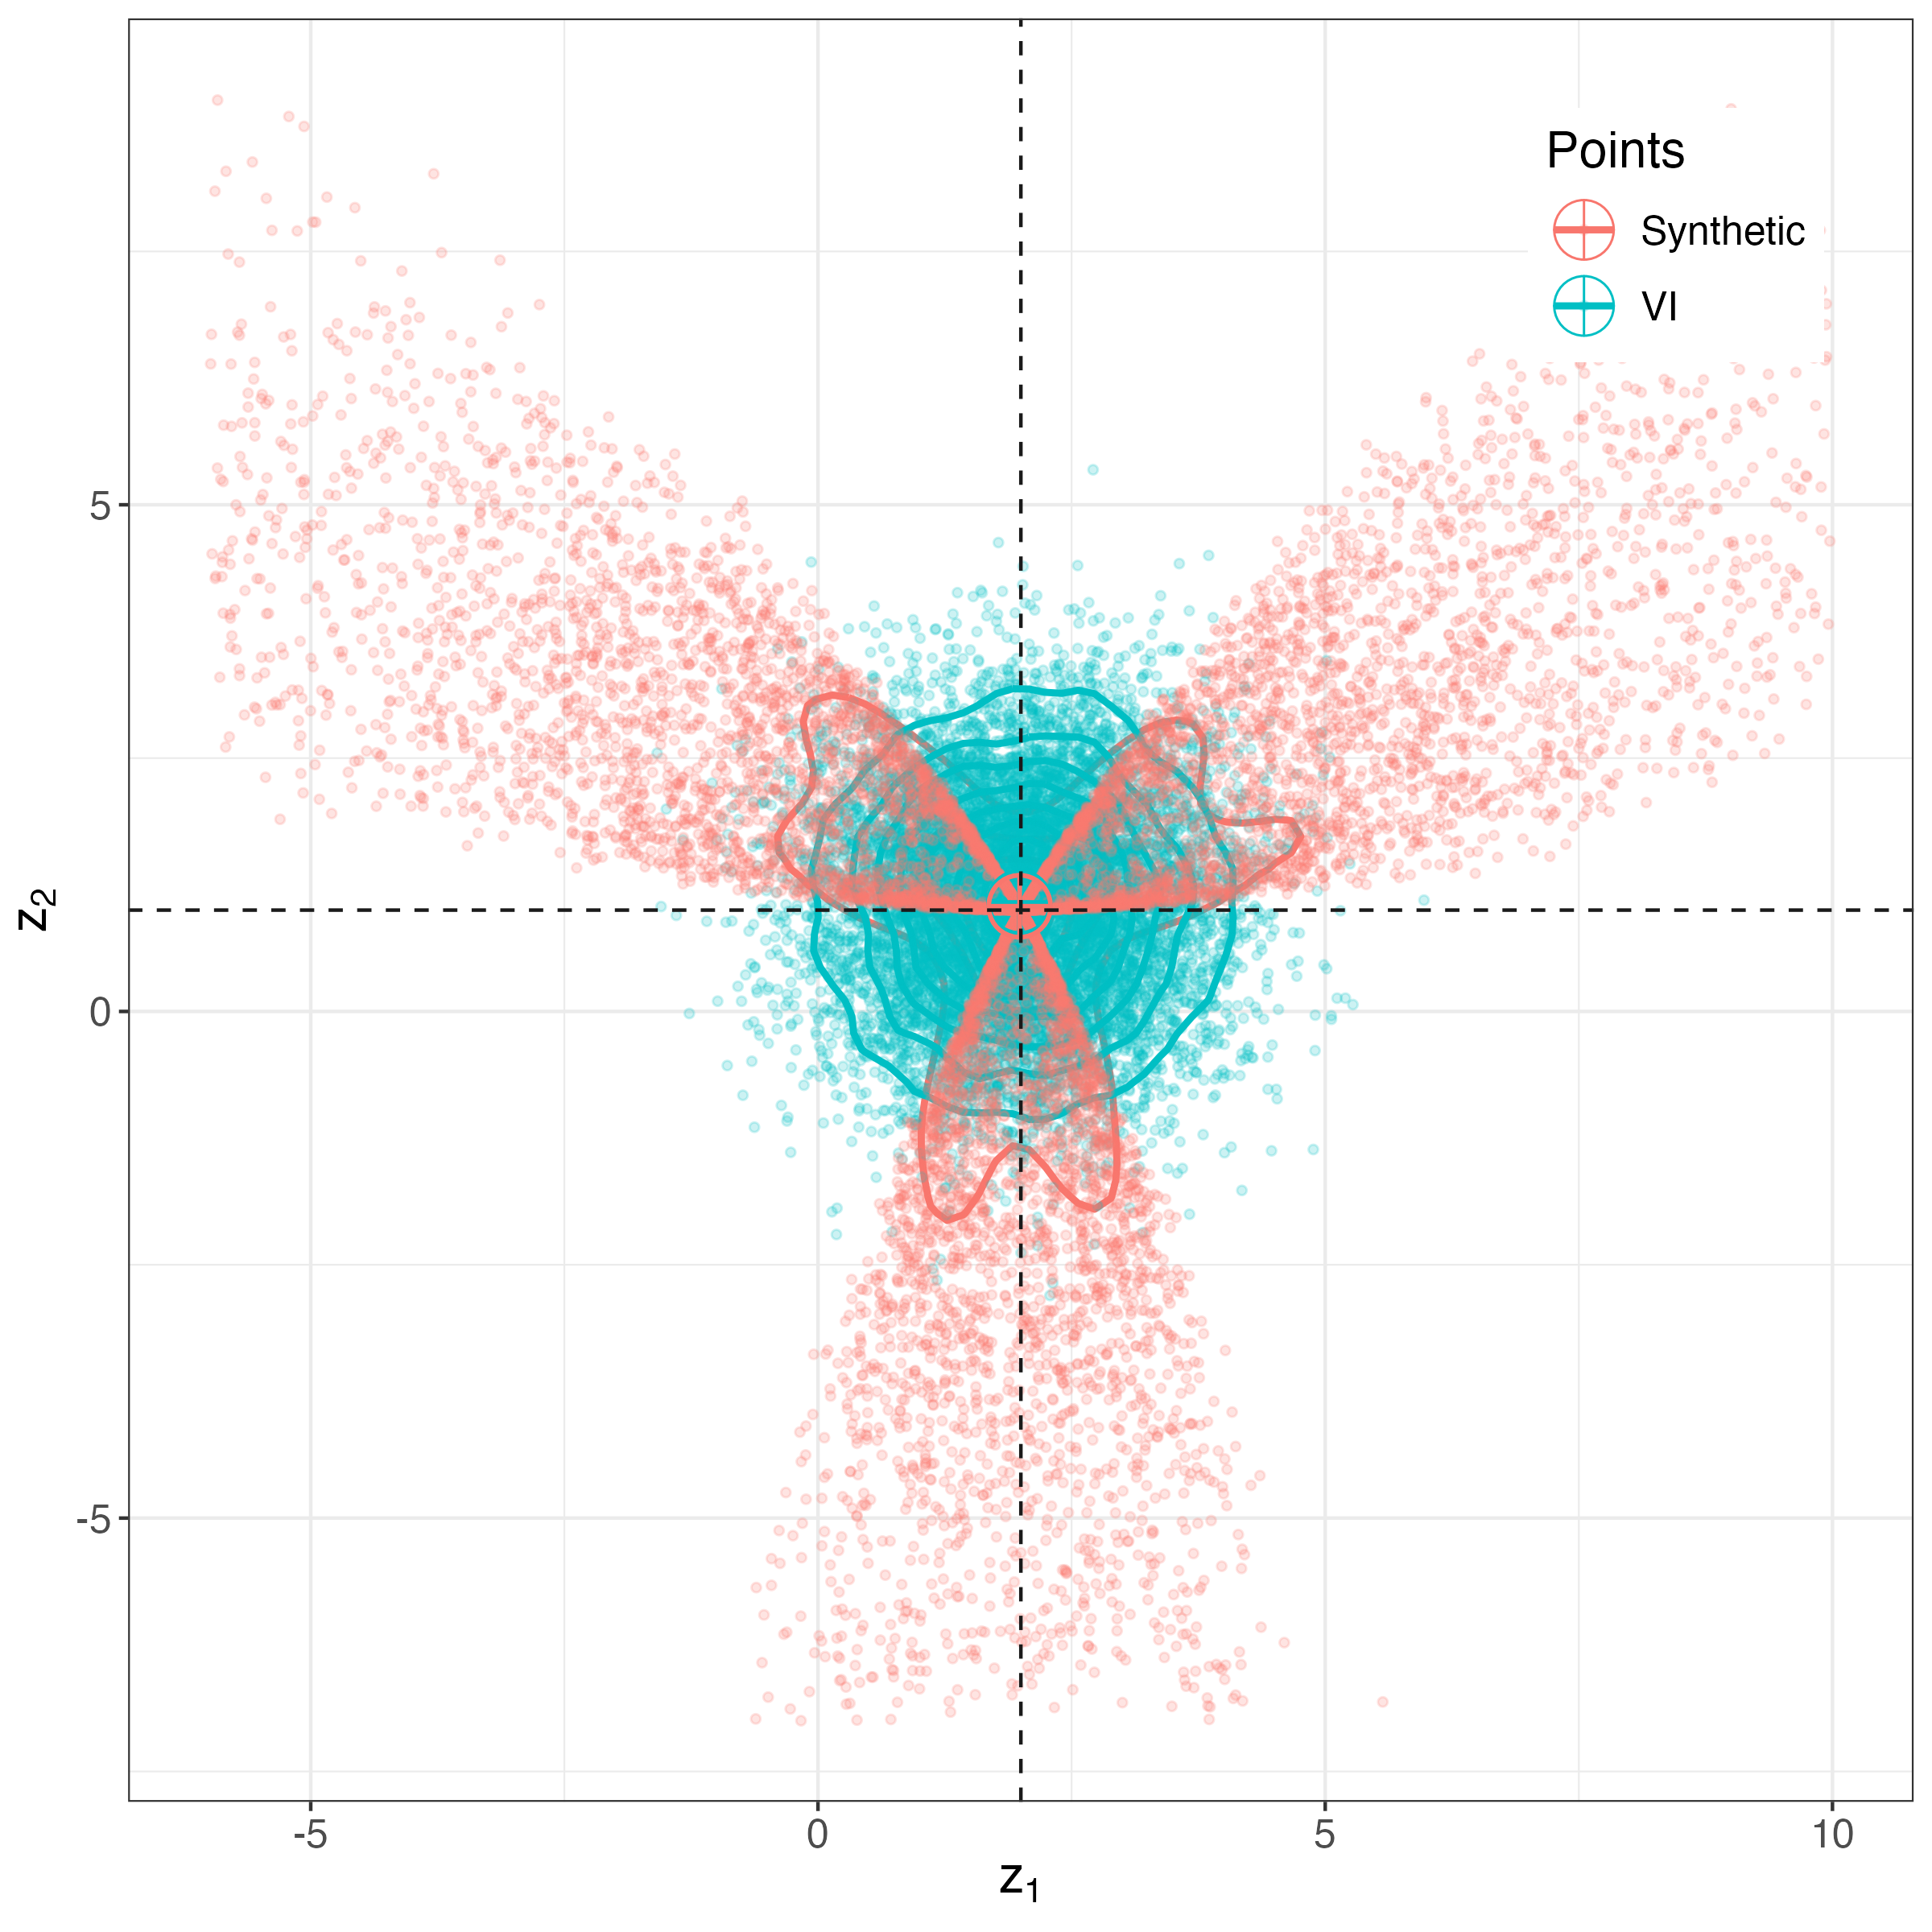
\includegraphics[width=\linewidth]{plots/VI_ex1.png}
        \caption{VI recovers the mean on a 3-rotationally symmetric target density}
    \end{minipage}
    \hfill
    \begin{minipage}{0.45\textwidth}
        \centering
        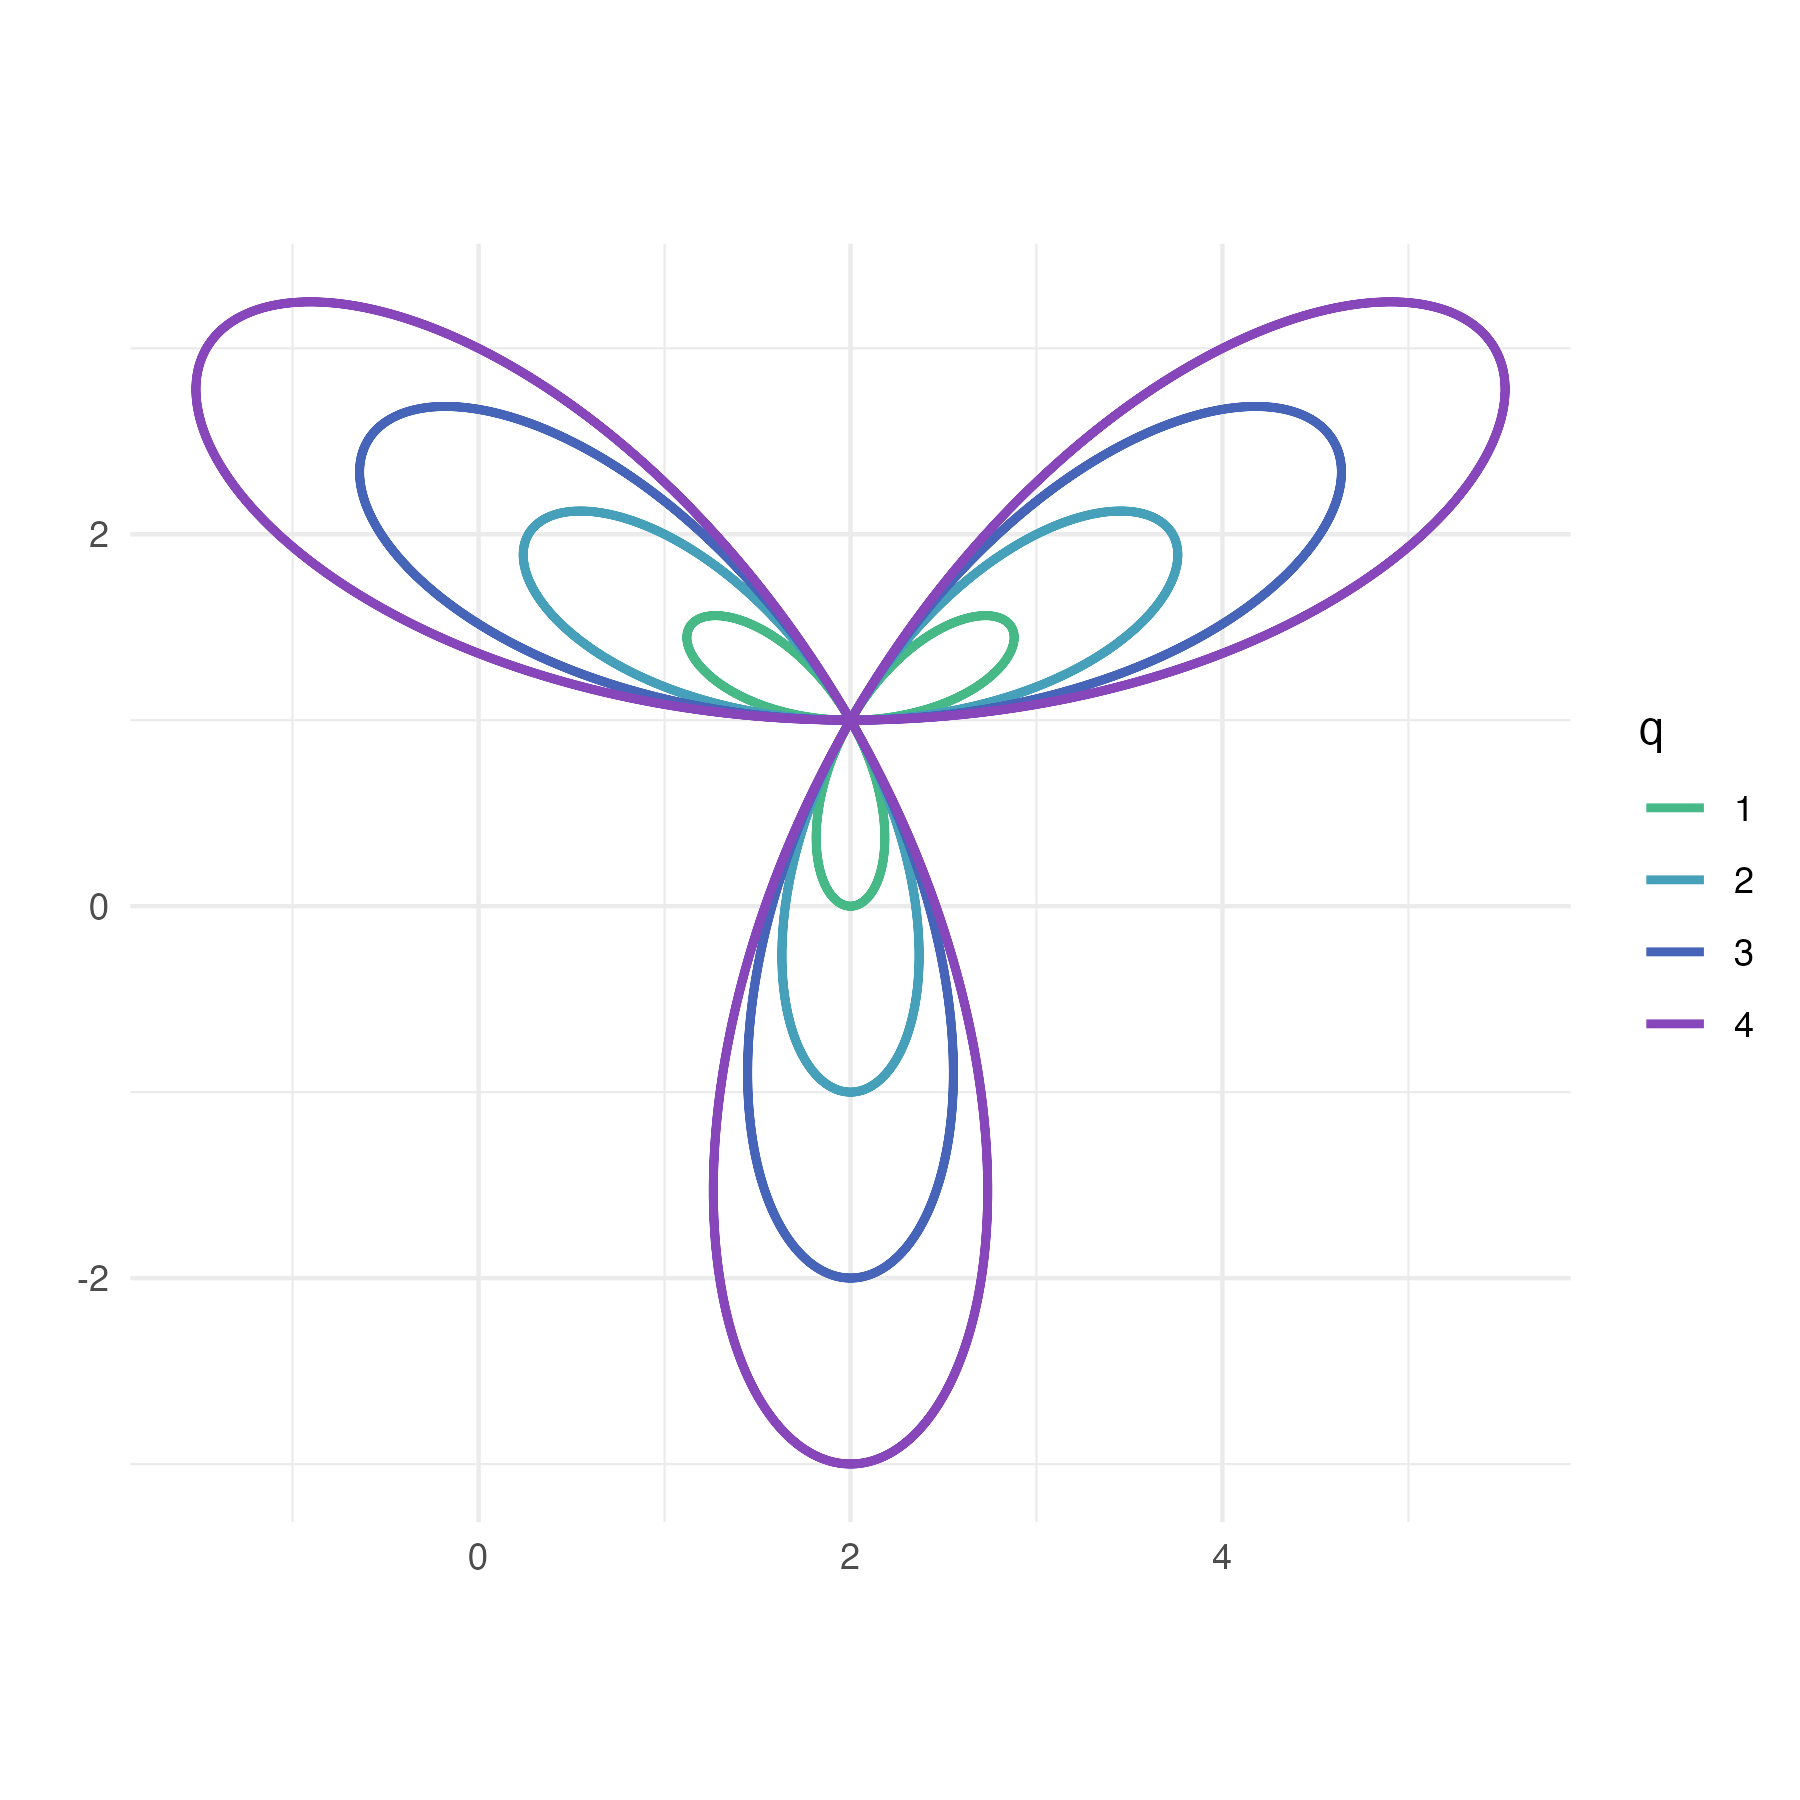
\includegraphics[width=\linewidth]{plots/level_curves_ex1.png}
        \caption{Level curves parametrized by $q$ and $\theta$}
    \end{minipage}
    \hfill
    \begin{minipage}{0.45\textwidth}
        \centering
        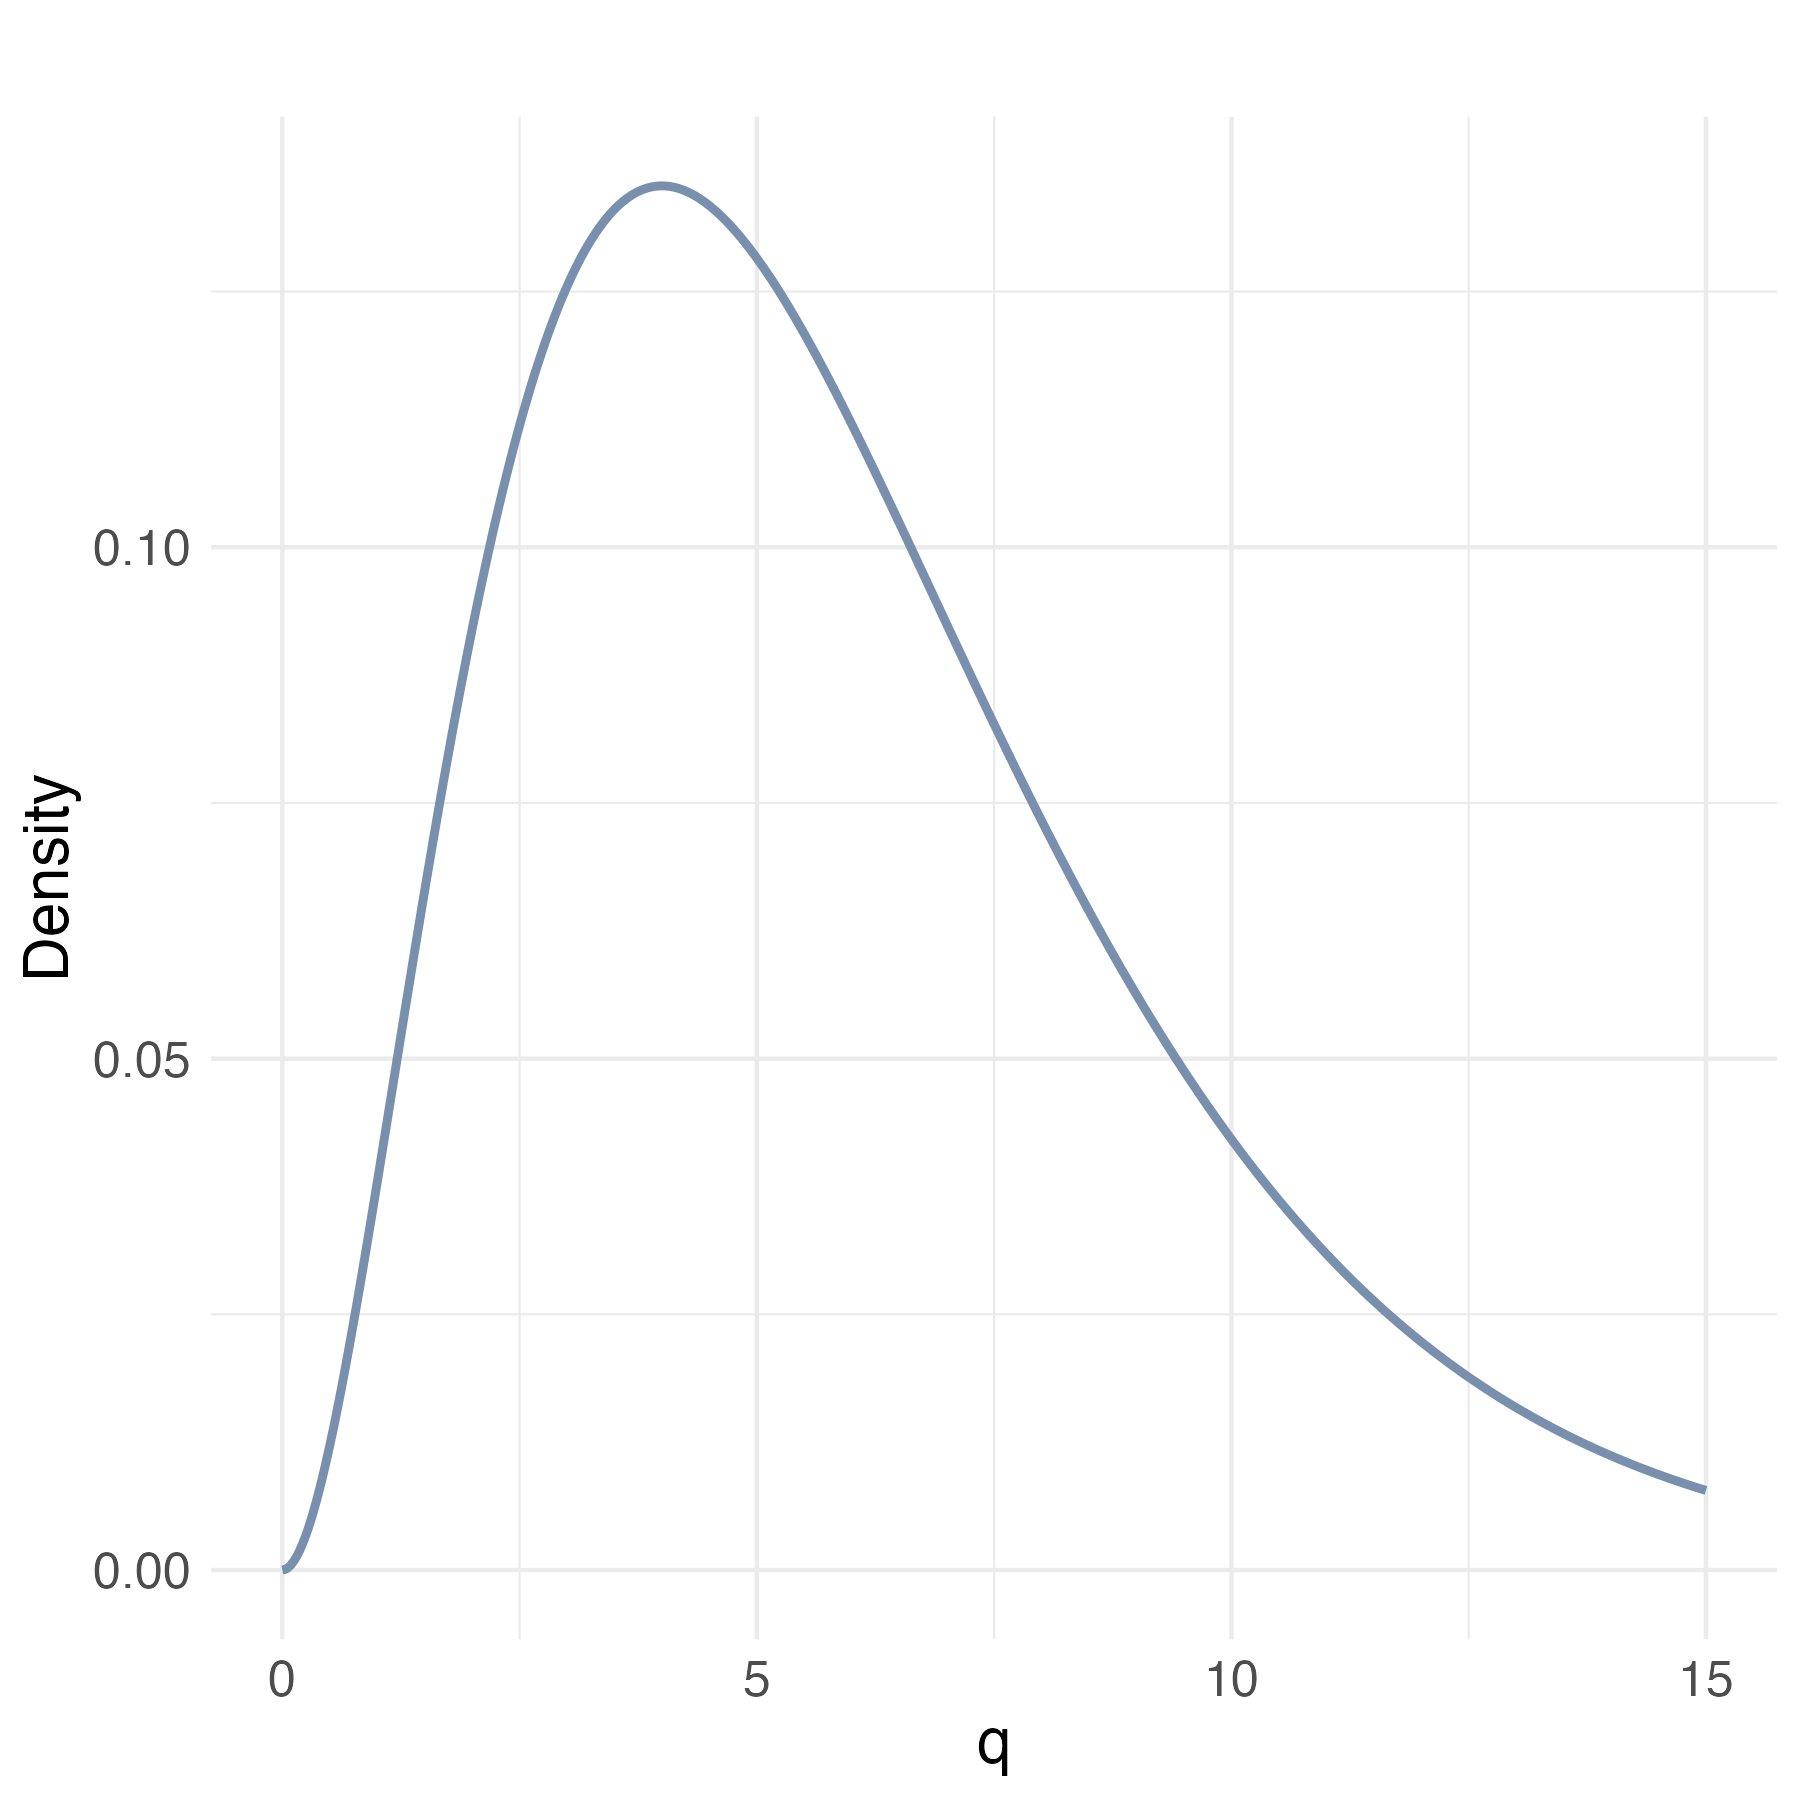
\includegraphics[width=\linewidth]{plots/density_q_ex1.png}
        \caption{Density of $q$}
    \end{minipage}
\end{figure}

\clearpage
\textbf{Target density 2:}
\begin{figure}[h!]
    \centering
    \begin{minipage}{0.6\textwidth}
        \centering
        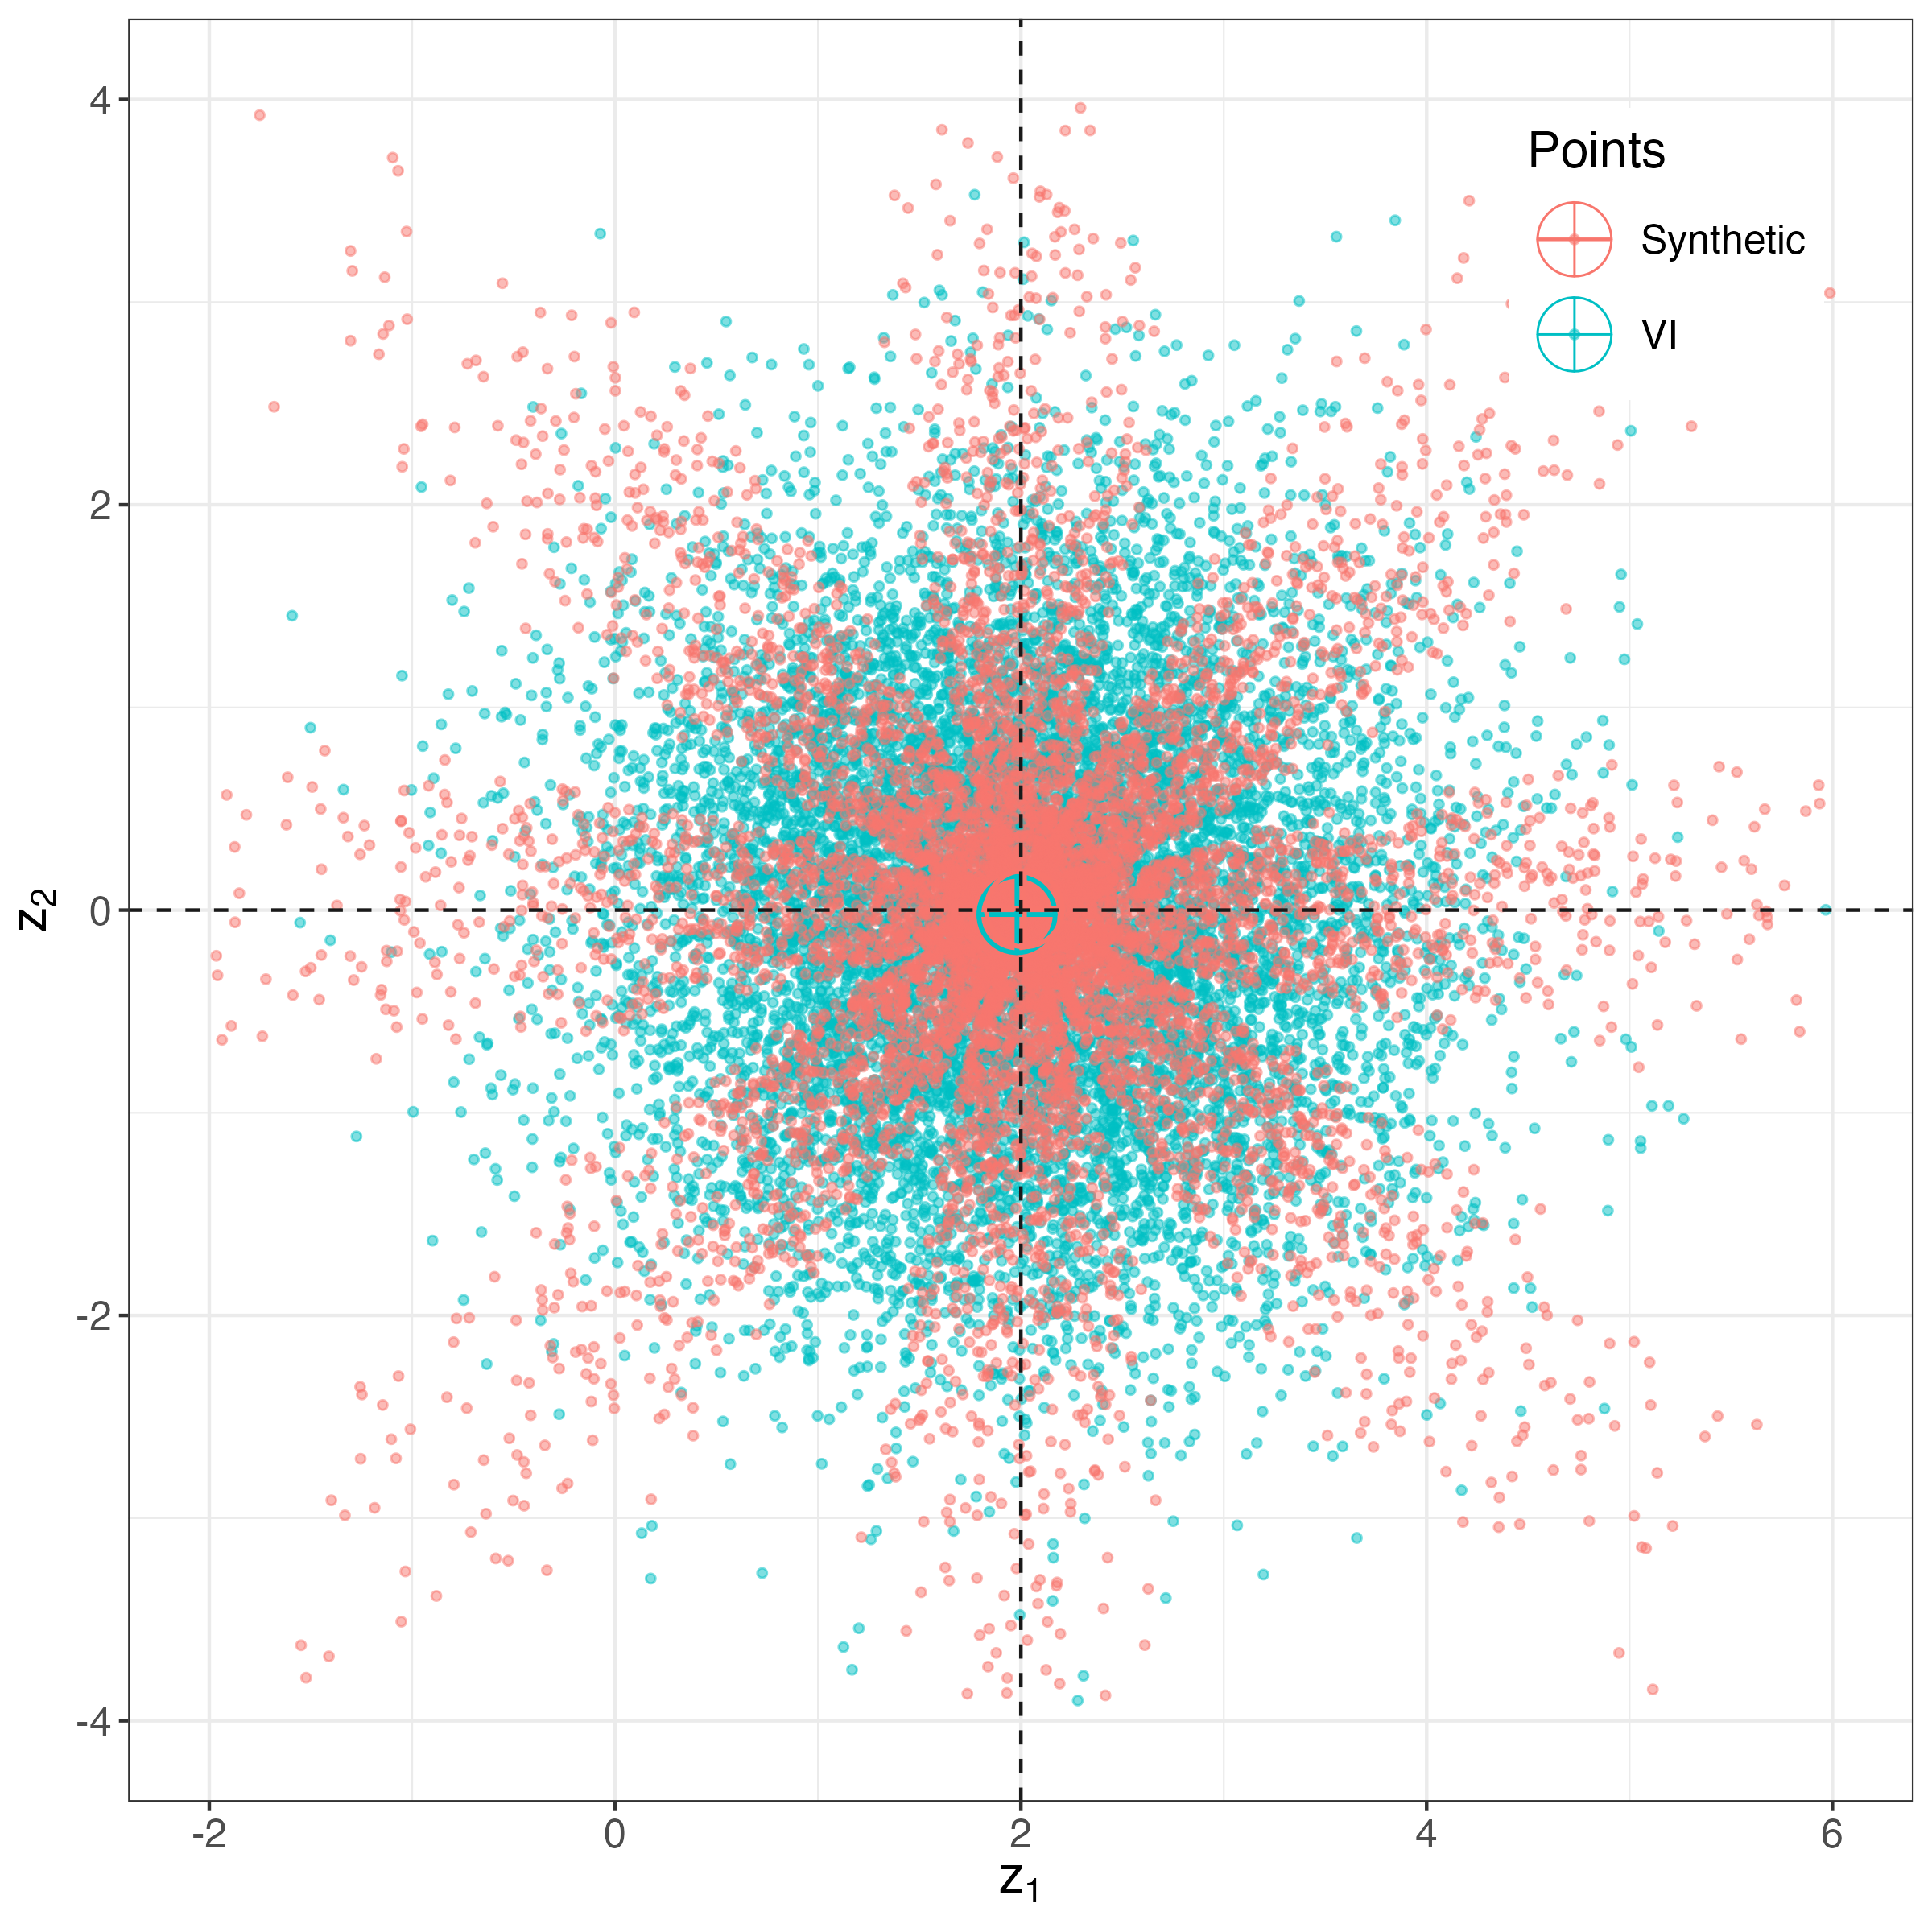
\includegraphics[width=\linewidth]{plots/VI_ex2.png}
        \caption{VI recovers the mean on an 8-rotationally symmetric target density}
    \end{minipage}
    \hfill
    \begin{minipage}{0.45\textwidth}
        \centering
        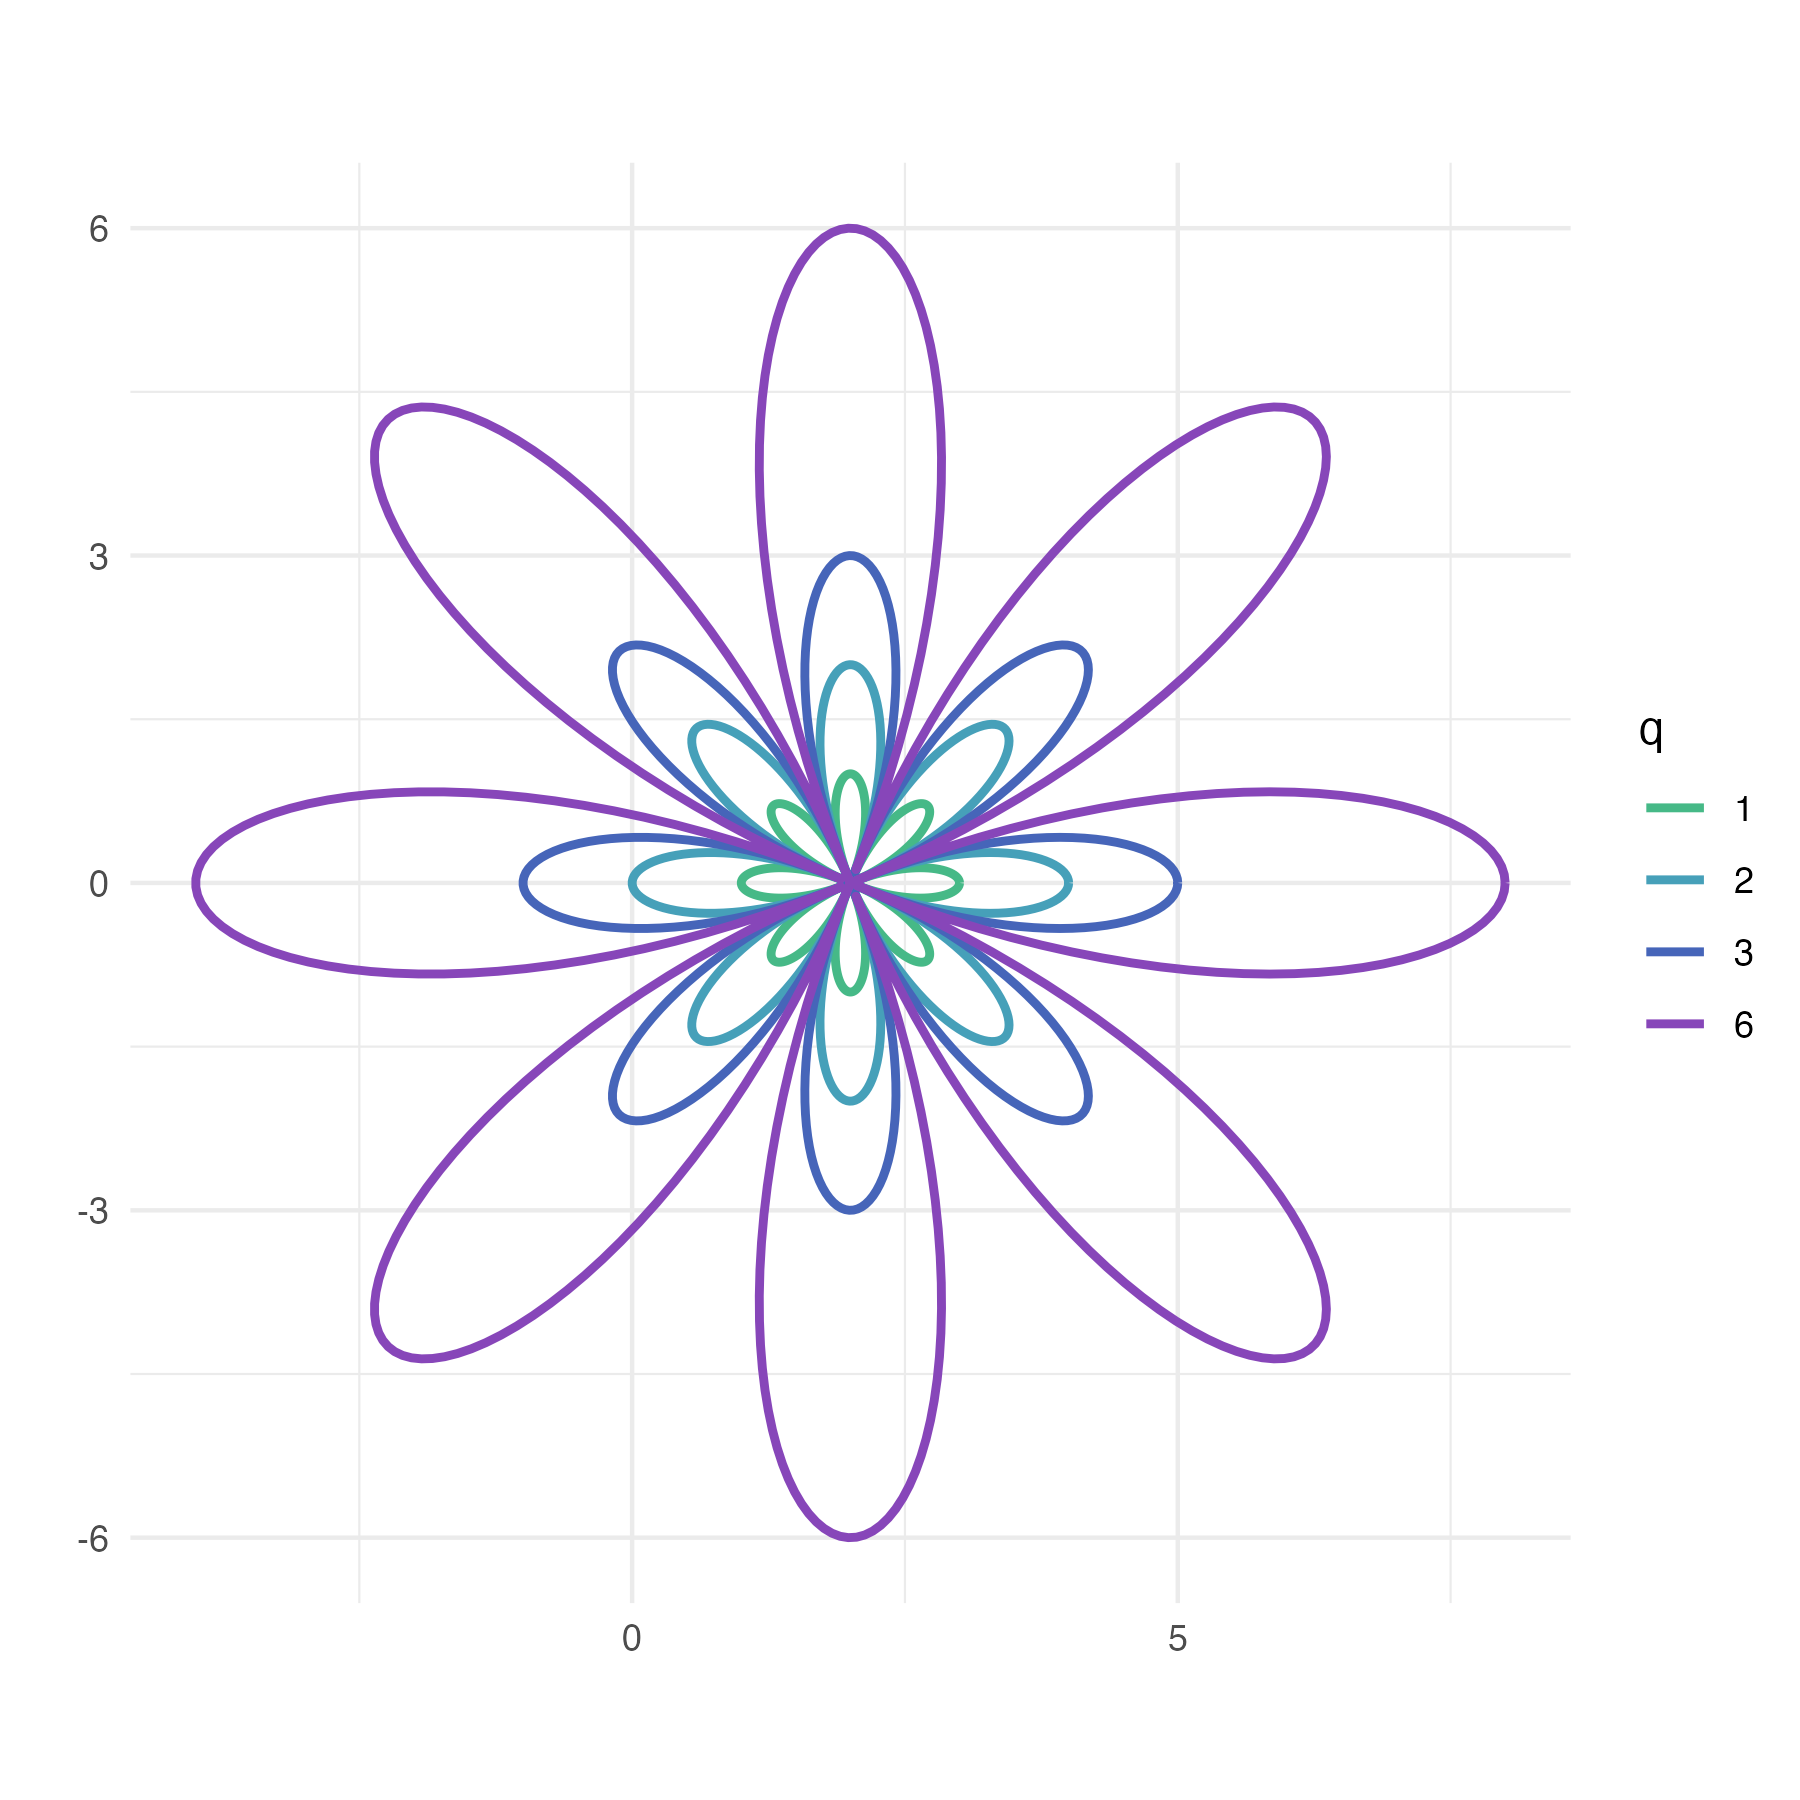
\includegraphics[width=\linewidth]{plots/level_curves_ex2.png}
        \caption{Level curves parametrized by $q$ and $\theta$}
    \end{minipage}
    \hfill
    \begin{minipage}{0.45\textwidth}
        \centering
        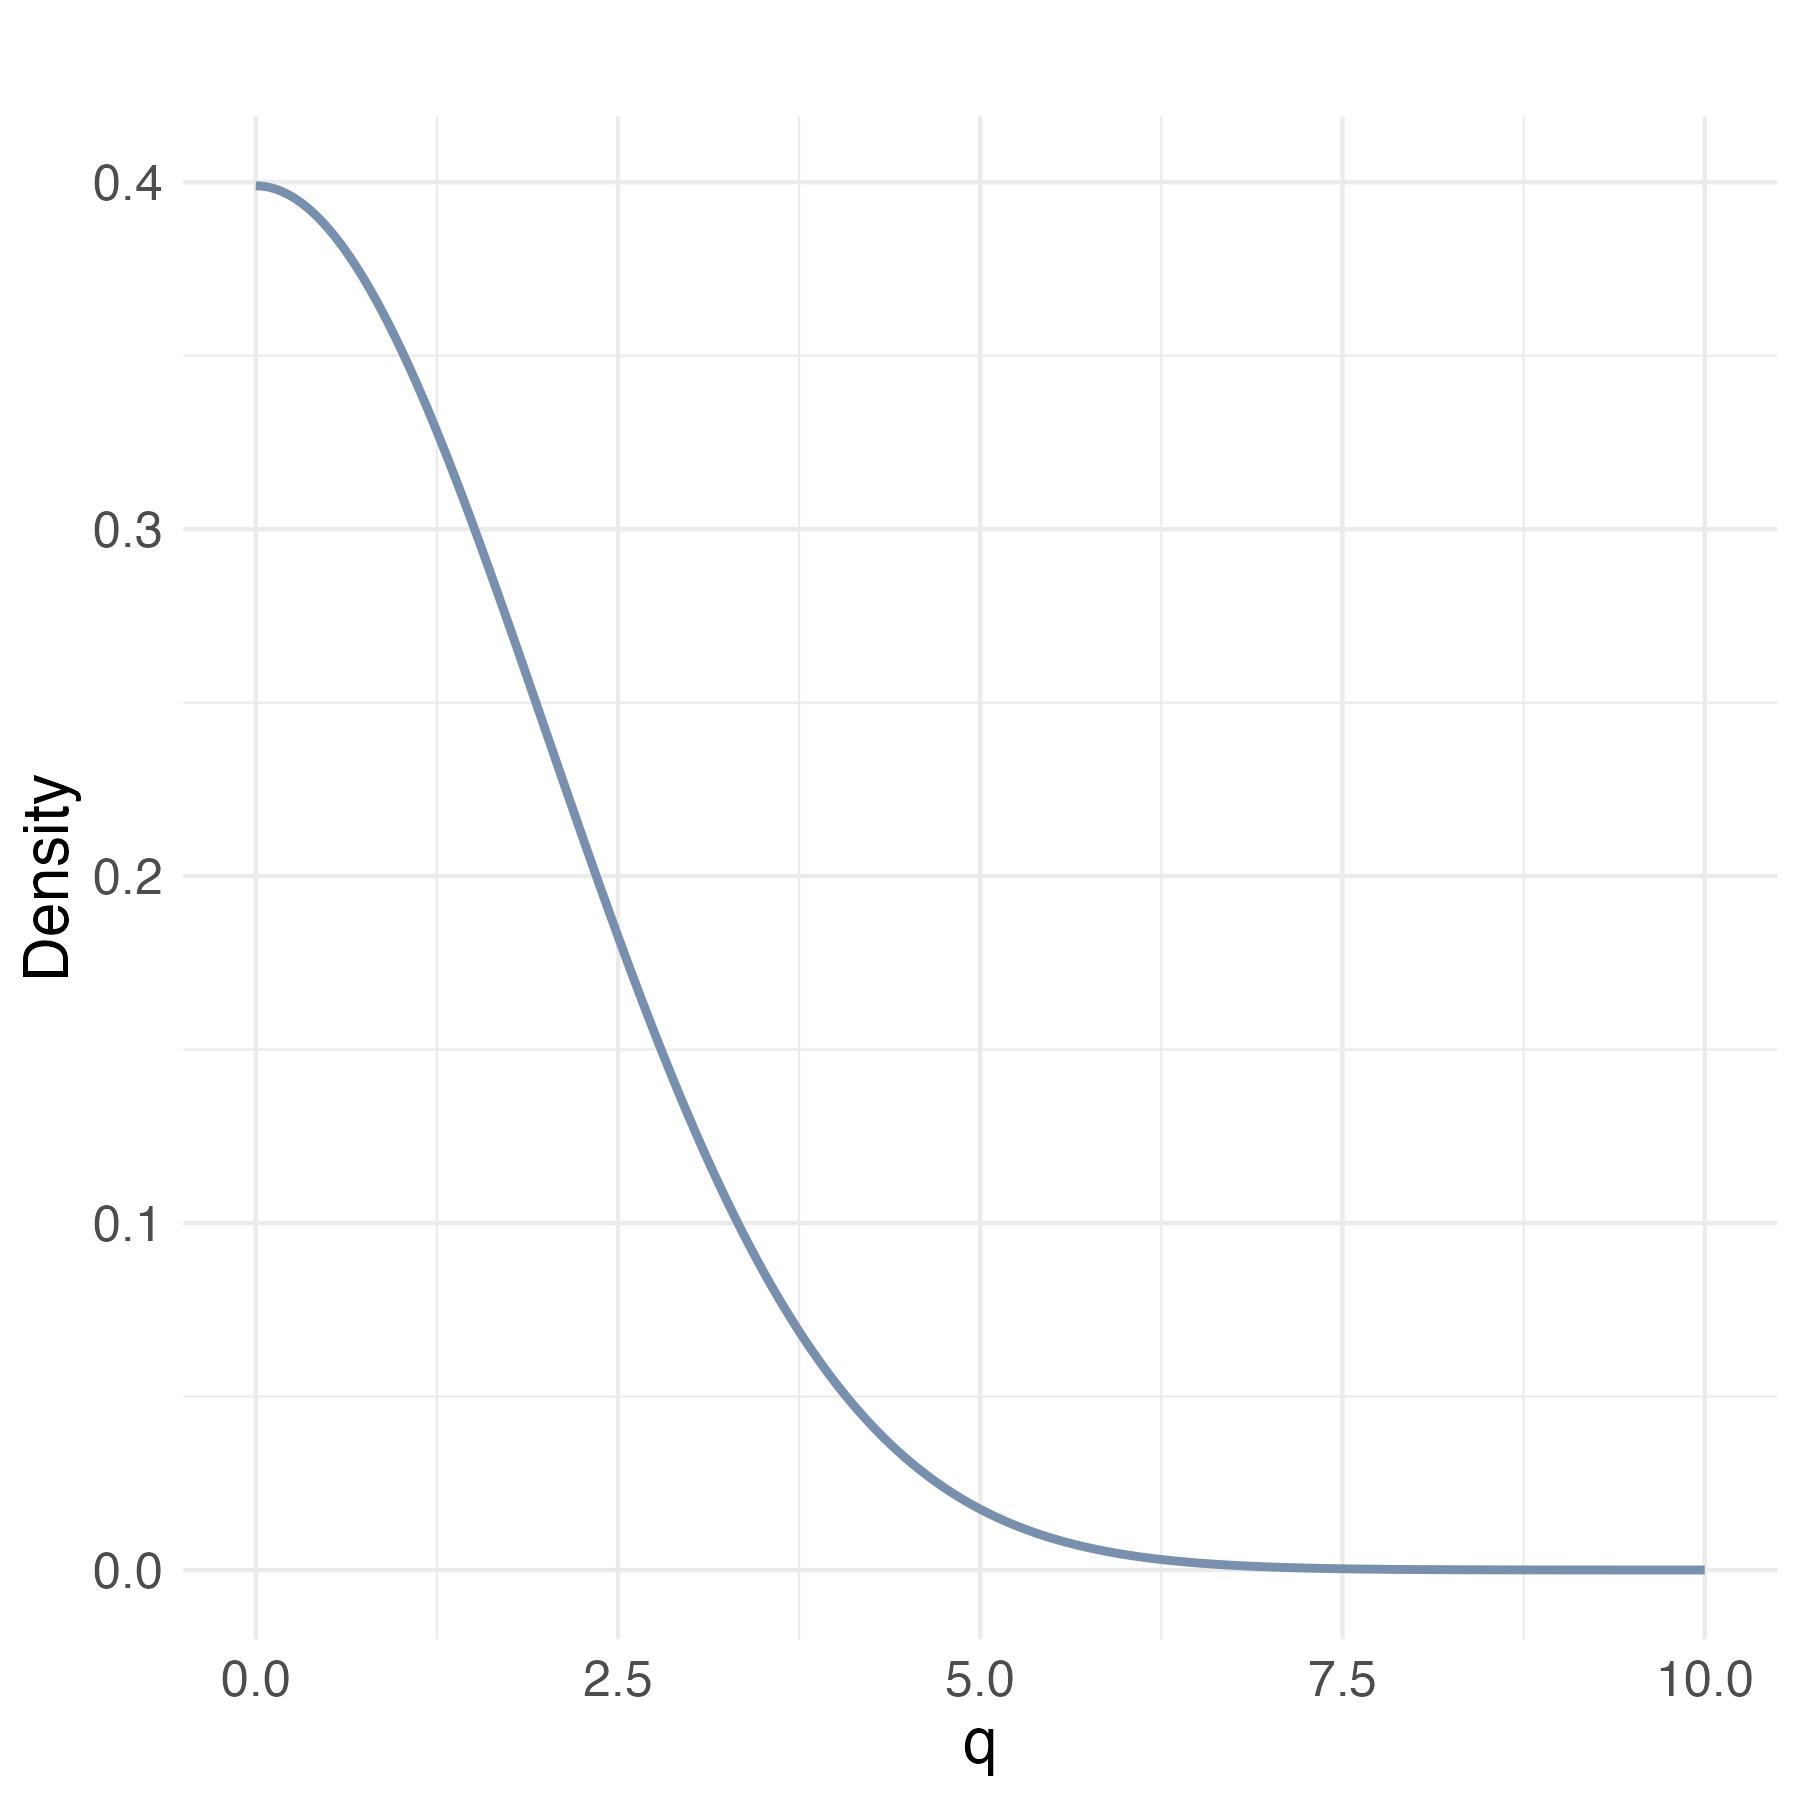
\includegraphics[width=\linewidth]{plots/density_q_ex2.png}
        \caption{Density of $q$}
    \end{minipage}
\end{figure}

\clearpage
\textbf{Target density 3:}
\begin{figure}[h!]
    \centering
    \begin{minipage}{0.6\textwidth}
        \centering
        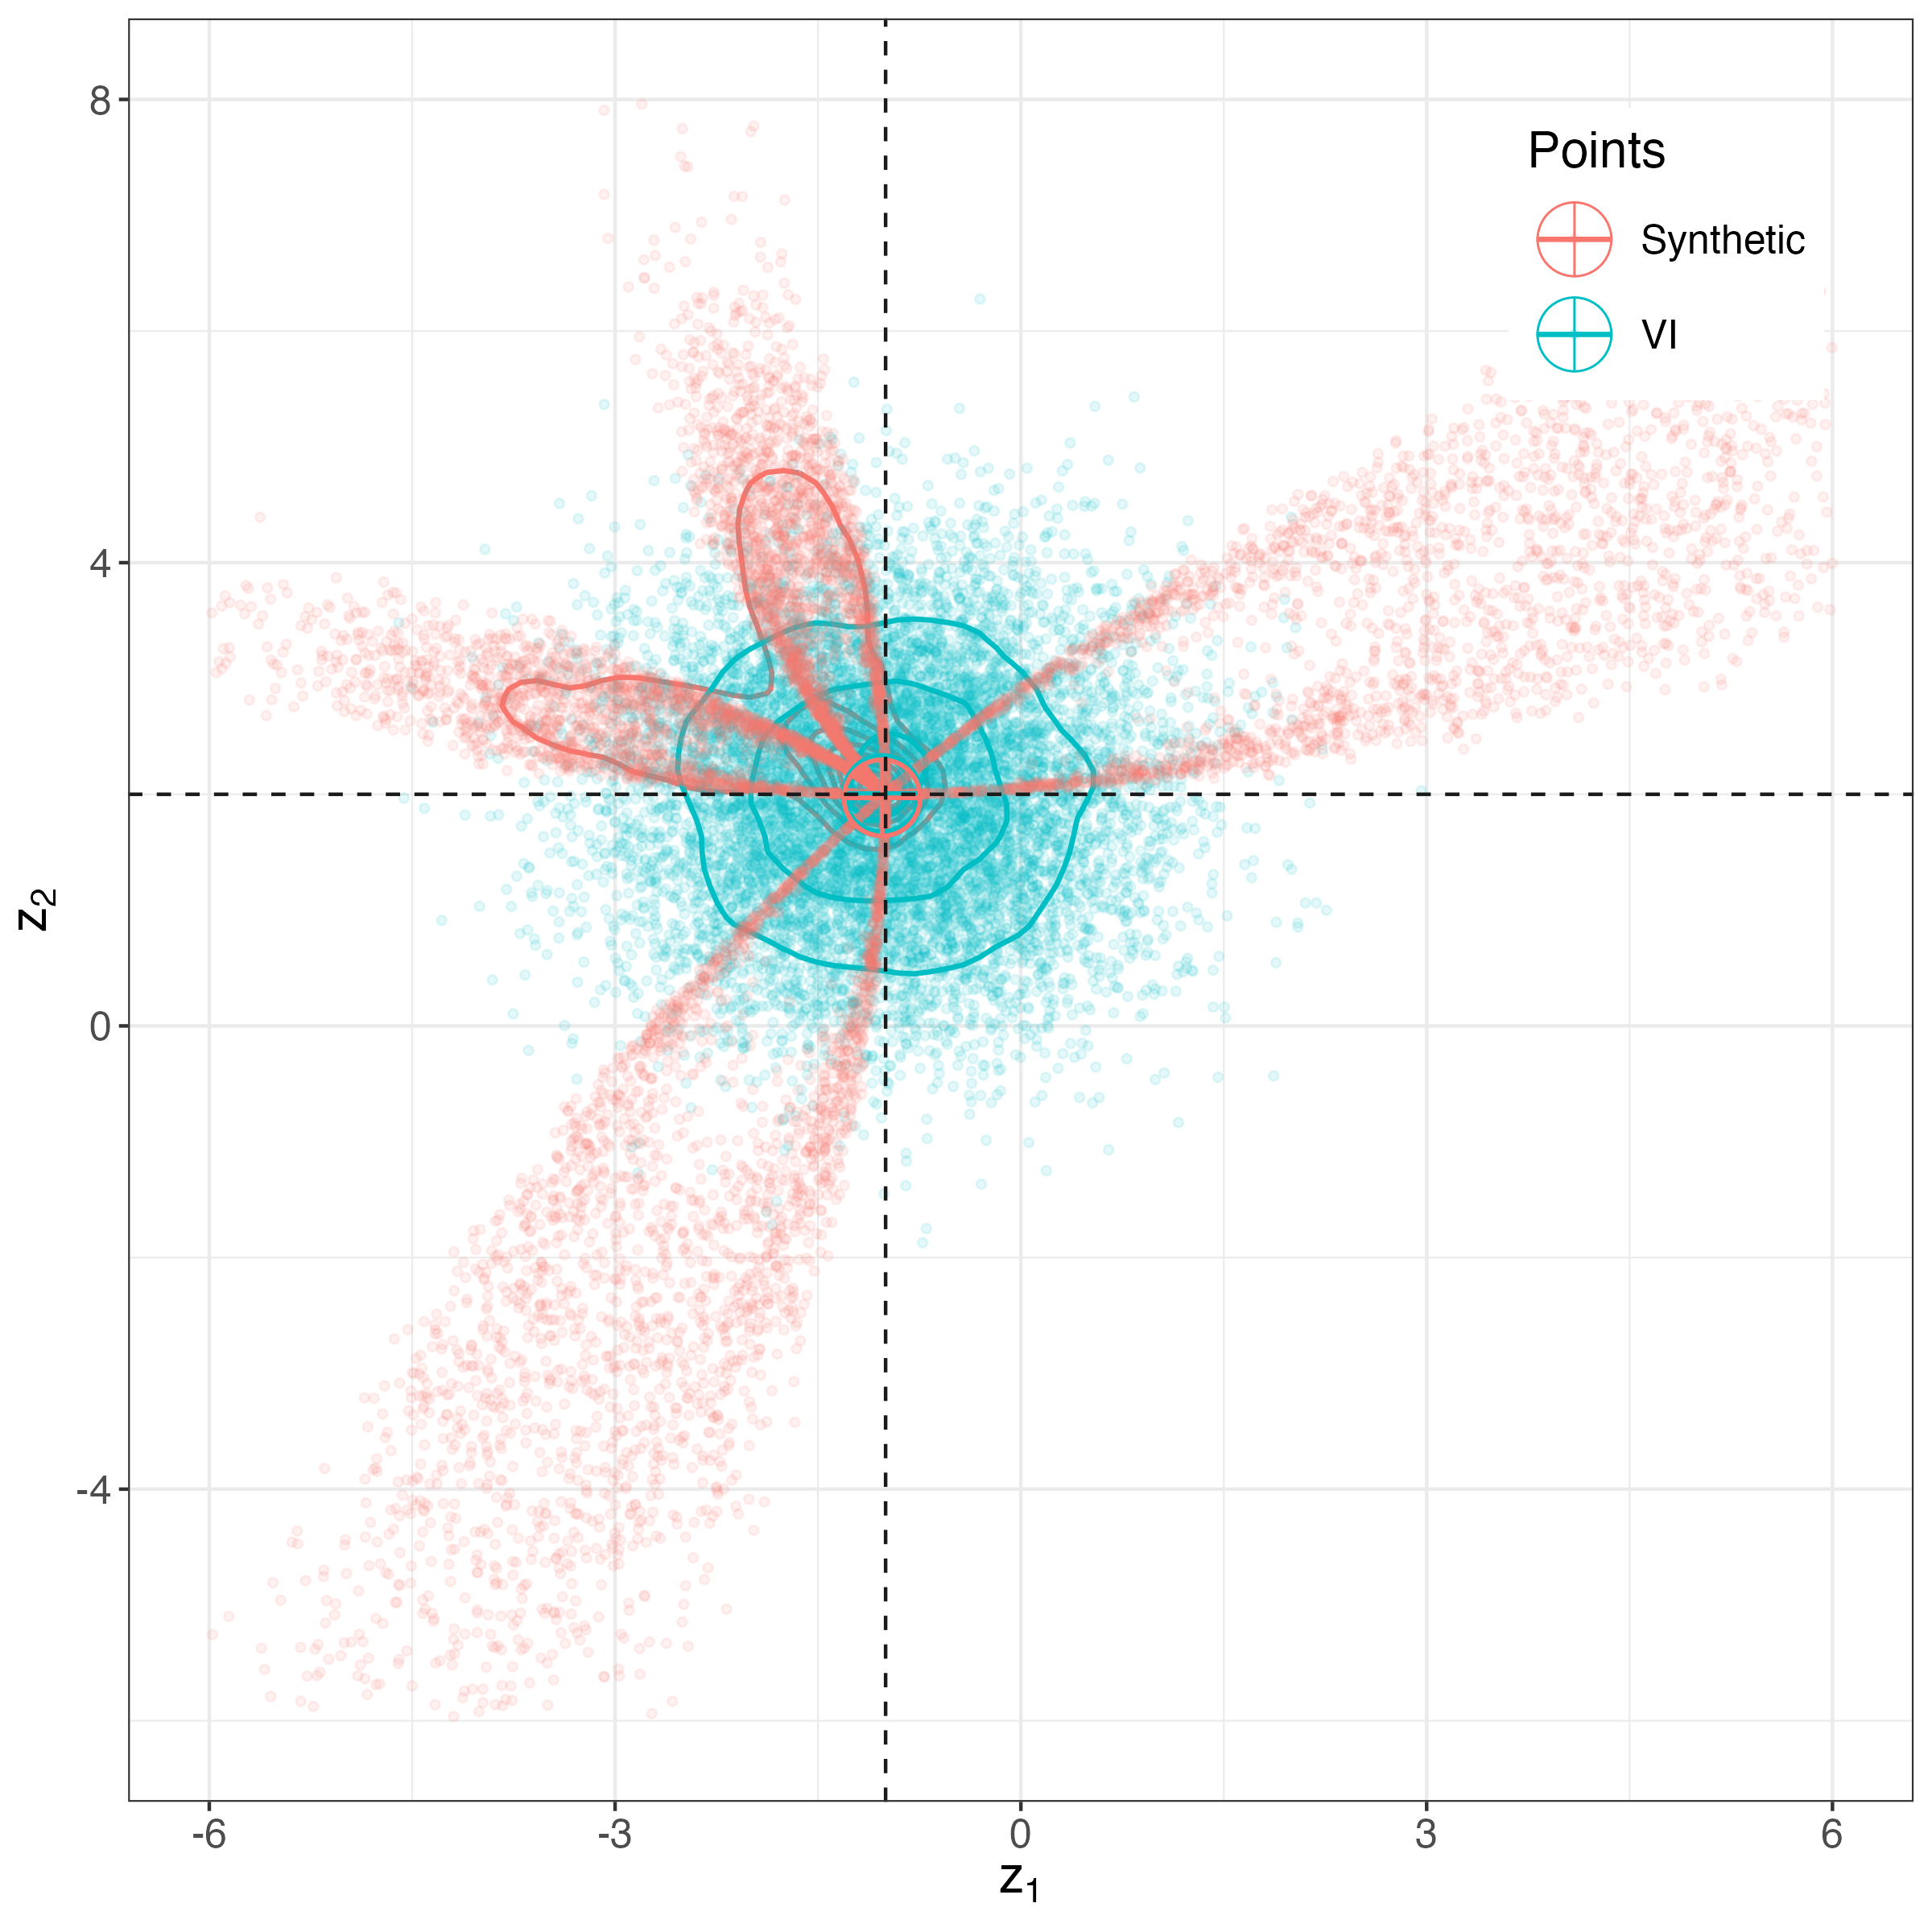
\includegraphics[width=\linewidth]{plots/VI_ex3.png}
        \caption{VI recovers the mean for a reflection-symmetric target}
    \end{minipage}
    \hfill
    \begin{minipage}{0.45\textwidth}
        \centering
        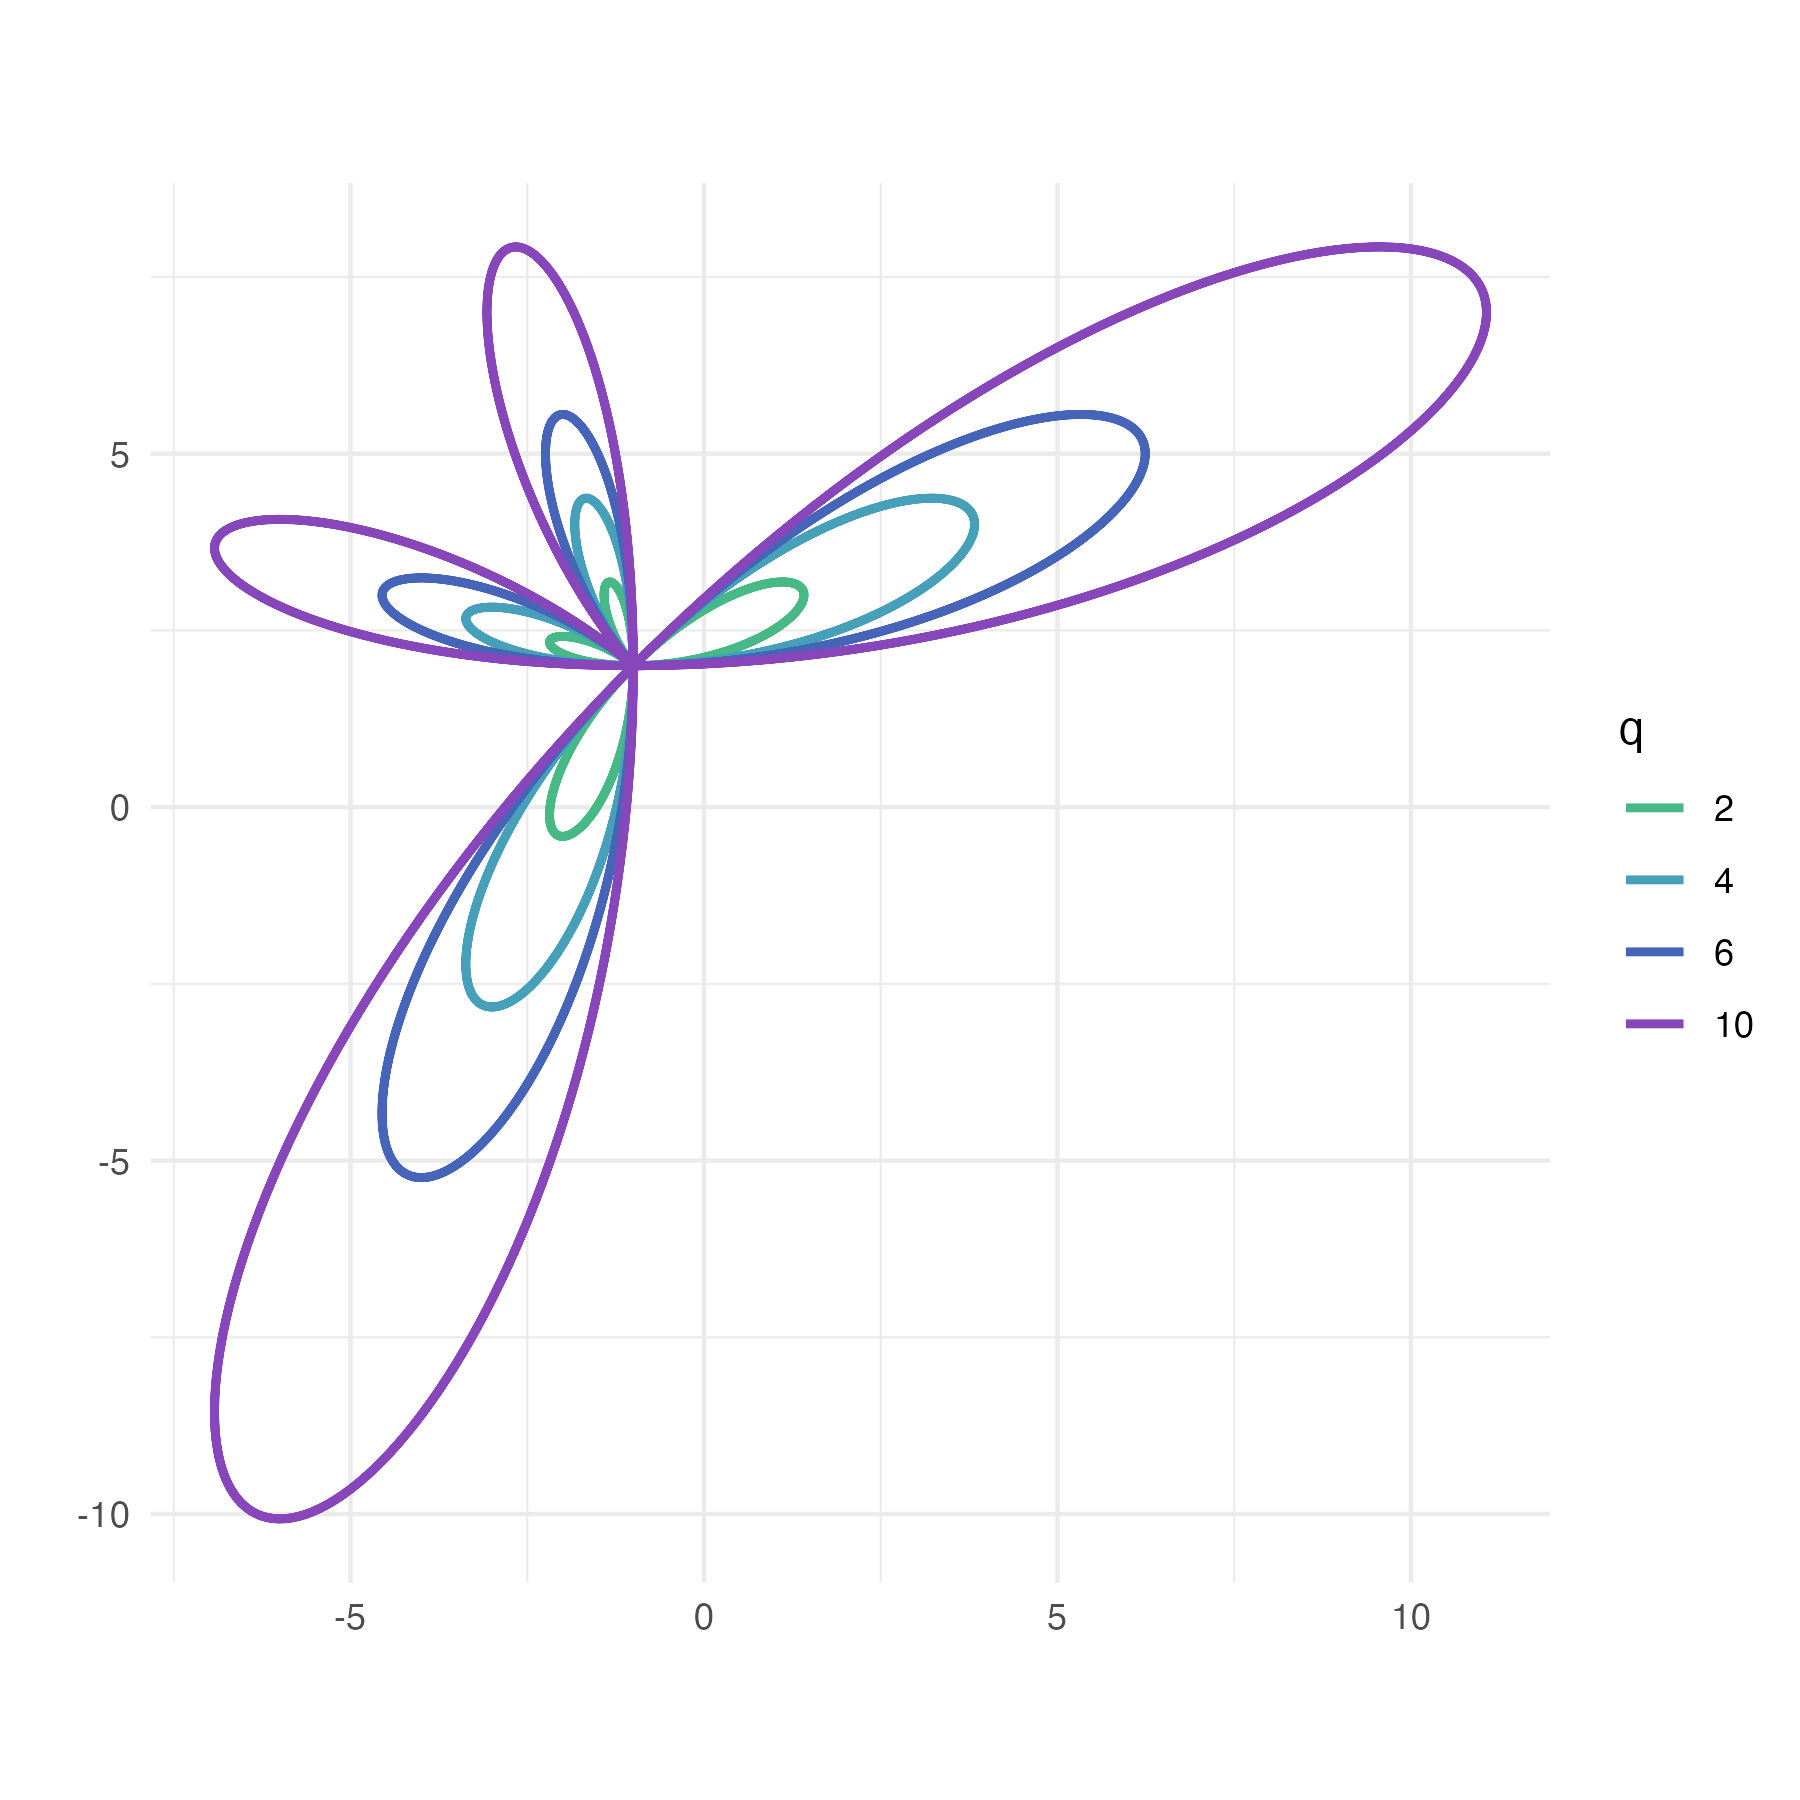
\includegraphics[width=\linewidth]{plots/level_curves_ex3.png}
        \caption{Level curves parametrized by $q$ and $\theta$}
    \end{minipage}
    \hfill
    \begin{minipage}{0.45\textwidth}
        \centering
        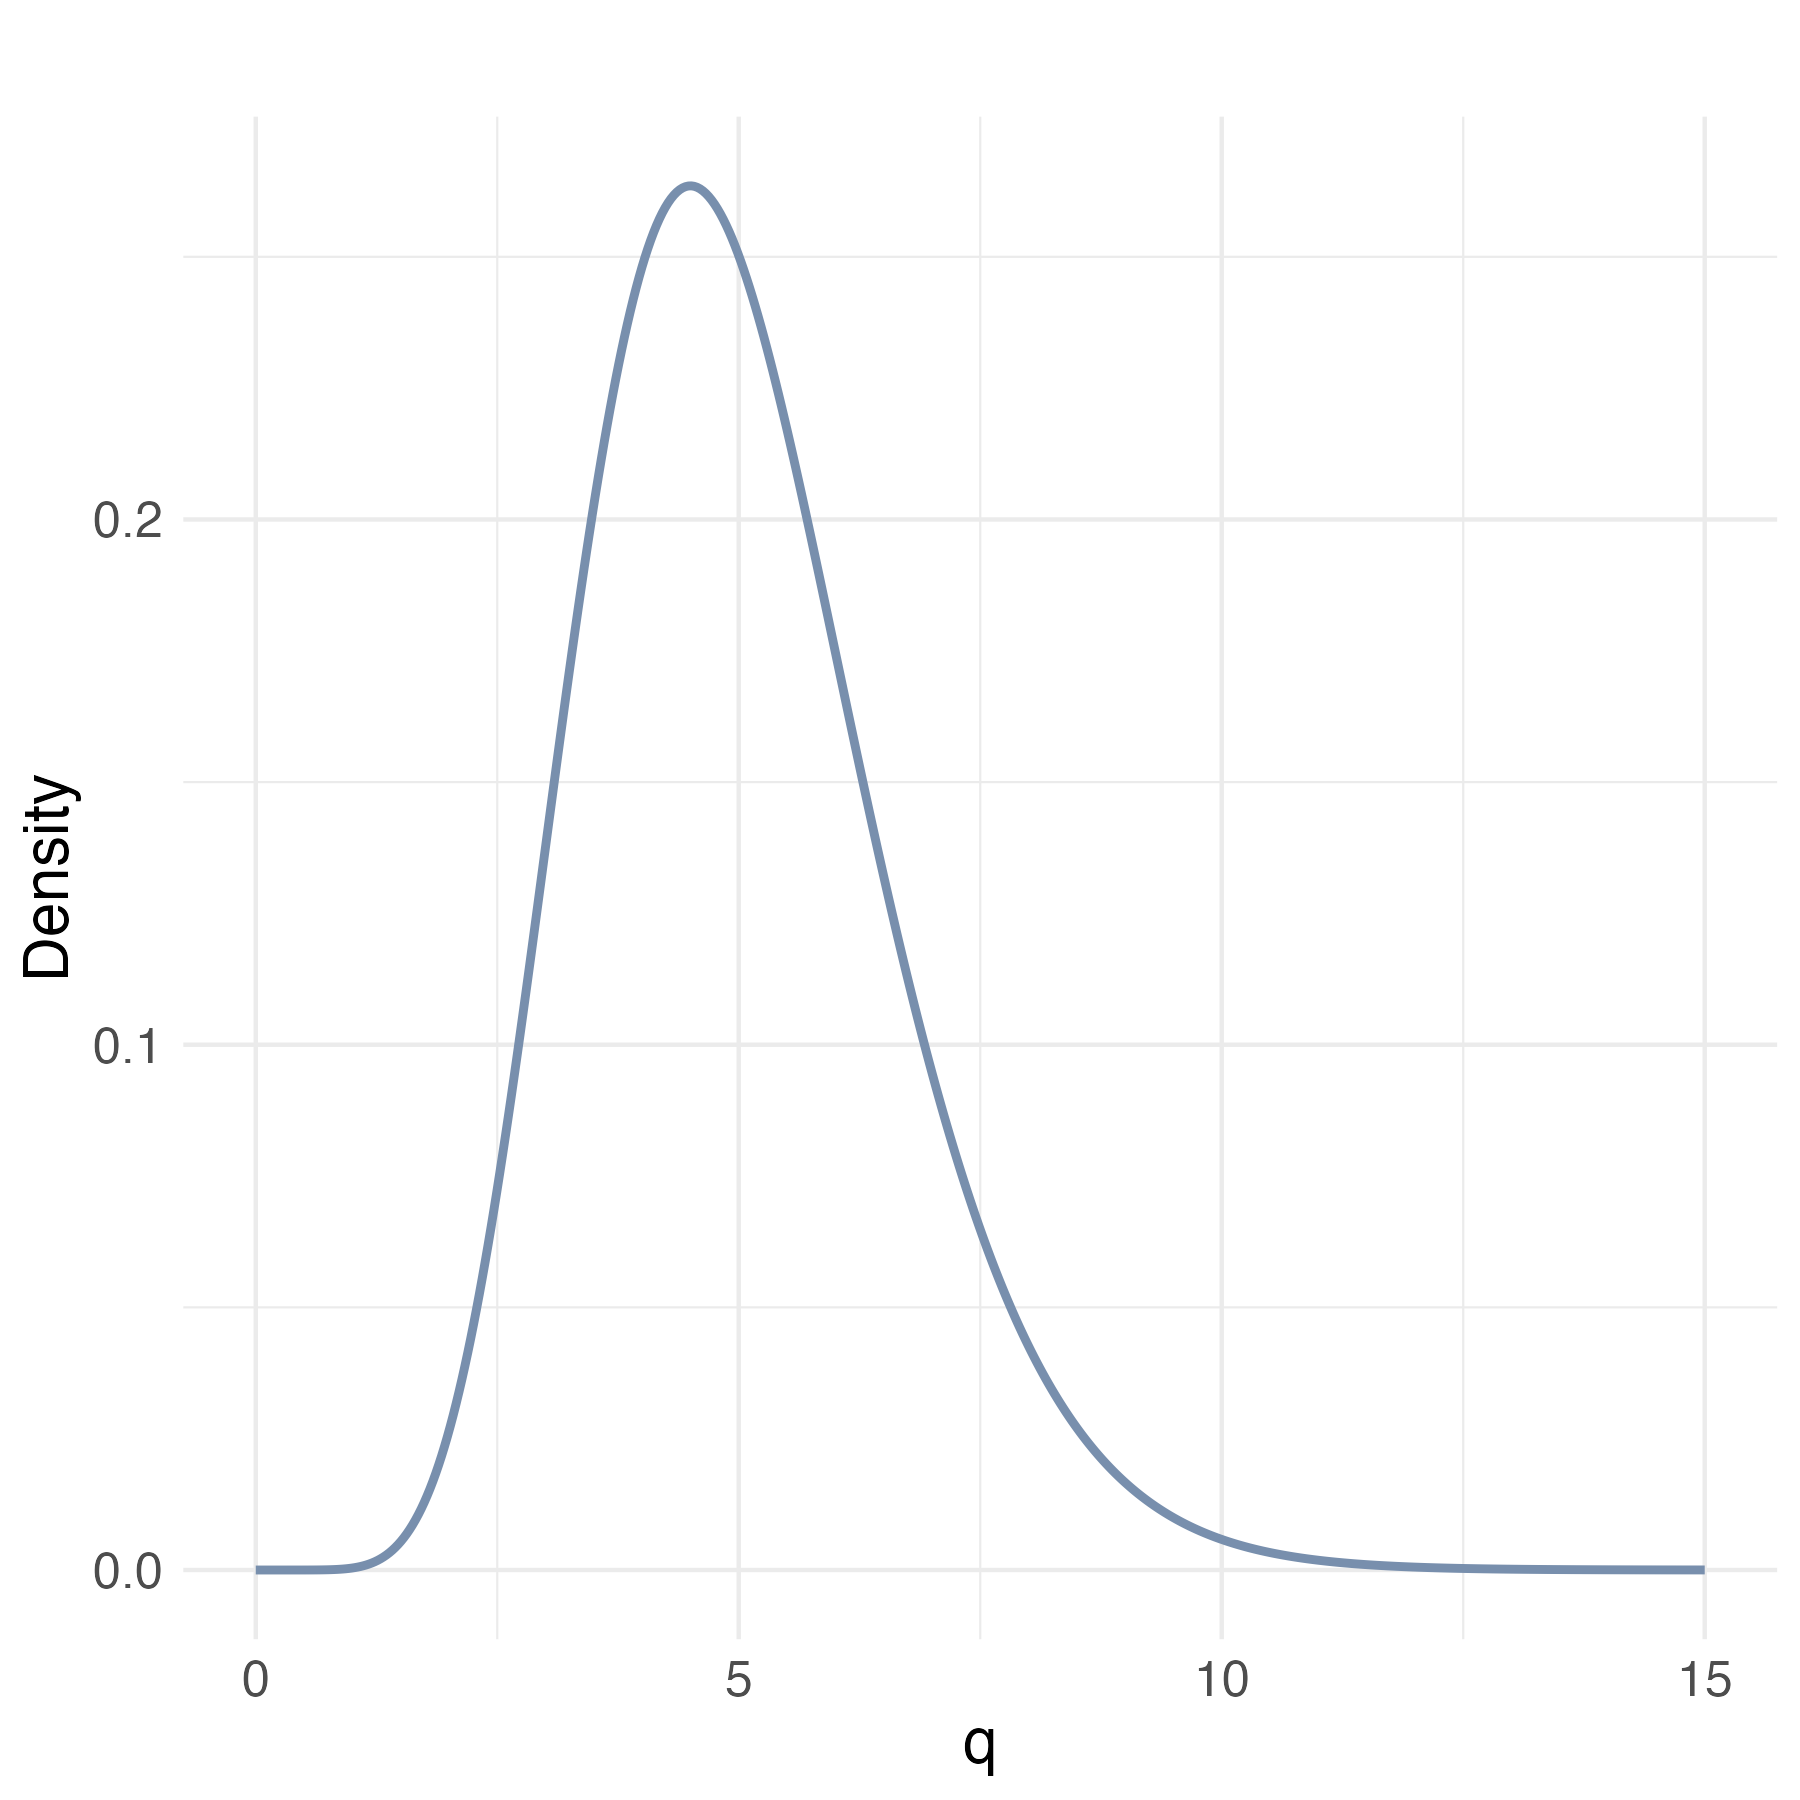
\includegraphics[width=\linewidth]{plots/density_q_ex3.png}
        \caption{Density of $q$}
    \end{minipage}
\end{figure}










% Bibliography
\clearpage
\addcontentsline{toc}{section}{Bibliography} % Adds "Bibliography" to the table of contents
\bibliographystyle{unsrt} % Other options are plain, unsrt, apalike
\bibliography{references}   % Look for references.bib

% References
% \clearpage
% \addcontentsline{toc}{section}{References}
% \bibliographystyle{unsrt}
% \bibliography{references5}

\end{document}